\documentclass{article}

\usepackage{fancyhdr}
\usepackage{wrapfig}
\usepackage{extramarks}
\usepackage{multicol}
\usepackage{amsmath}
\usepackage{amsthm}
\usepackage{amsfonts}
\usepackage{tikz}
\usepackage[plain]{algorithm}
\usepackage{algpseudocode}
\usepackage{enumerate}
\usepackage[shortlabels]{enumitem}                                          
                    \setlist[enumerate, 1]{1\textsuperscript{o}}



\usepackage{listings}
\usepackage{xcolor}
\lstset { %
    language=C++,
    backgroundcolor=\color{black!5}, % set backgroundcolor
    basicstyle=\footnotesize,% basic font setting
}

%\usetikzlibrary{automata,positioning}
\usetikzlibrary{positioning,shapes,shadows,arrows,automata}

%
% Basic Document Settings
%

\topmargin=-0.45in
\evensidemargin=0in
\oddsidemargin=0in
\textwidth=6.5in
\textheight=9.0in
\headsep=0.25in

\linespread{1.1}

\pagestyle{fancy}
\lhead{\hmwkClass}
\chead{ (\hmwkClassInstructor\ \hmwkClassTime) }
\rhead{\shortName \hspace{0.4cm} \hmwkTitle}
\lfoot{\lastxmark}
\cfoot{\thepage}

\renewcommand\headrulewidth{0.4pt}
\renewcommand\footrulewidth{0.4pt}

\setlength\parindent{0pt}

%
% Create Problem Sections
%

\newcommand{\enterProblemHeader}[1]{
    \nobreak\extramarks{}{Problem \arabic{#1} continued on next page\ldots}\nobreak{}
    \nobreak\extramarks{Problem \arabic{#1} (continued)}{Problem \arabic{#1} continued on next page\ldots}\nobreak{}
}

\newcommand{\exitProblemHeader}[1]{
    \nobreak\extramarks{Problem \arabic{#1} (continued)}{Problem \arabic{#1} continued on next page\ldots}\nobreak{}
    \stepcounter{#1}
    \nobreak\extramarks{Problem \arabic{#1}}{}\nobreak{}
}

\setcounter{secnumdepth}{0}
\newcounter{partCounter}
\newcounter{homeworkProblemCounter}
\setcounter{homeworkProblemCounter}{1}
\nobreak\extramarks{Problem \arabic{homeworkProblemCounter}}{}\nobreak{}

%
% Homework Problem Environment
%
% This environment takes an optional argument. When given, it will adjust the
% problem counter. This is useful for when the problems given for your
% assignment aren't sequential. See the last 3 problems of this template for an
% example.
%
\newenvironment{homeworkProblem}[1][-1]{
    \ifnum#1>0
        \setcounter{homeworkProblemCounter}{#1}
    \fi
    \section{Problem \arabic{homeworkProblemCounter}}
    \setcounter{partCounter}{1}
    \enterProblemHeader{homeworkProblemCounter}
}{
    \exitProblemHeader{homeworkProblemCounter}
}

%
% Homework Details
%   - Title
%   - Due date
%   - Class
%   - Section/Time
%   - Instructor
%   - Author
%

\newcommand{\hmwkTitle}{Homework\ \#1}
\newcommand{\hmwkDueDate}{January 20 2015}
\newcommand{\hmwkClass}{CS581 Theory of Computation}
\newcommand{\hmwkClassTime}{Winter 2016}
\newcommand{\hmwkClassInstructor}{Harry H. Porter}
\newcommand{\hmwkAuthorName}{Konstantin Macarenco}
\newcommand{\shortName}{Konstantin M.}

%
% Title Page
%

\title{
    \vspace{2in}
    \textmd{\textbf{\hmwkClass:\ \hmwkTitle}}\\
    \normalsize\vspace{0.1in}\small{Due\ on\ \hmwkDueDate\ at 2:00pm}\\
    \vspace{0.1in}\large{\textit{\hmwkClassInstructor\ \hmwkClassTime}}
    \vspace{3in}
}

\author{\textbf{\hmwkAuthorName}}
\date{}

\renewcommand{\part}[1]{\textbf{\large Part \Alph{partCounter}}\stepcounter{partCounter}\\}
\newcommand{\answ}[1]{\hspace{1cm}\textbf{Answ:} #1}
\newcommand{\problem}[1]{\large{\textbf{Problem #1} \\}}

%
% Various Helper Commands
%

% Useful for algorithms
\newcommand{\alg}[1]{\textsc{\bfseries \footnotesize #1}}

% For derivatives
\newcommand{\deriv}[1]{\frac{\mathrm{d}}{\mathrm{d}x} (#1)}

% For partial derivatives
\newcommand{\pderiv}[2]{\frac{\partial}{\partial #1} (#2)}

% Integral dx
\newcommand{\dx}{\mathrm{d}x}

% Alias for the Solution section header
\newcommand{\solution}{\textbf{\large Solution}}

% Probability commands: Expectation, Variance, Covariance, Bias
\newcommand{\E}{\mathrm{E}}
\newcommand{\Var}{\mathrm{Var}}
\newcommand{\Cov}{\mathrm{Cov}}
\newcommand{\Bias}{\mathrm{Bias}}

\begin{document}

\maketitle

\pagebreak

\large{\textbf{Problem 1.1} \\

The following are the state diagrams of two DFAs, $M_1$ and $M_2$. Answer the following 
questions about each of these machines.

\begin{center}
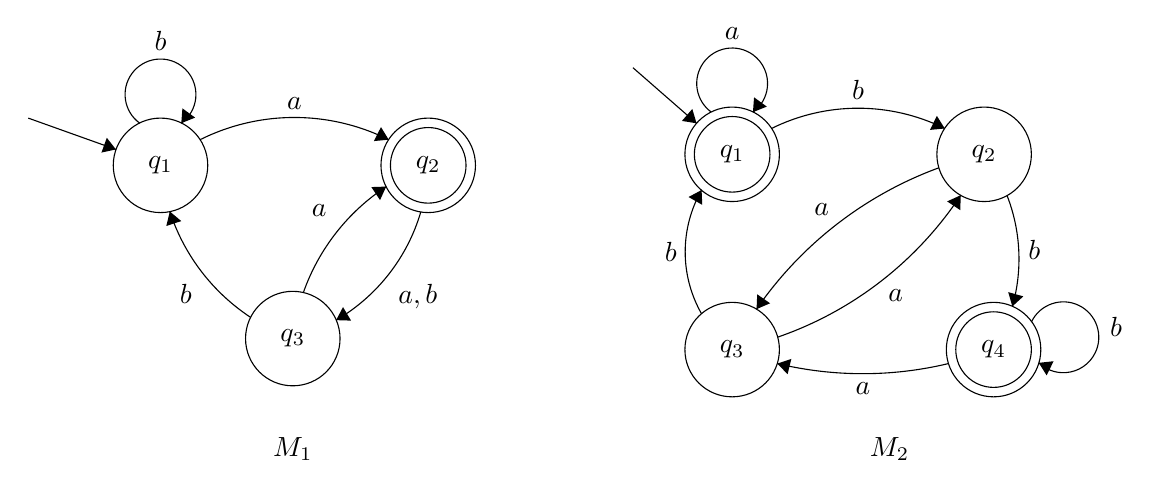
\begin{tikzpicture}[scale=0.2]
\tikzstyle{every node}+=[inner sep=0pt]
\draw [black] (9.8,-10.1) circle (3);
\draw (9.8,-10.1) node {$q_1$};
\draw [black] (26.8,-10.1) circle (3);
\draw (26.8,-10.1) node {$q_2$};
\draw [black] (26.8,-10.1) circle (2.4);
\draw [black] (18.2,-21.1) circle (3);
\draw (18.2,-21.1) node {$q_3$};
\draw (18.2,-28.1) node {$M_1$};
\draw [black] (46.1,-9.4) circle (3);
\draw (46.1,-9.4) node {$q_1$};
\draw [black] (46.1,-9.4) circle (2.4);
\draw [black] (62.1,-9.4) circle (3);
\draw (62.1,-9.4) node {$q_2$};
\draw [black] (46.1,-21.8) circle (3);
\draw (46.1,-21.8) node {$q_3$};
\draw (56.1,-28.1) node {$M_2$};
\draw [black] (62.7,-21.8) circle (3);
\draw (62.7,-21.8) node {$q_4$};
\draw [black] (62.7,-21.8) circle (2.4);
\draw [black] (8.477,-7.42) arc (234:-54:2.25);
\draw (9.8,-2.85) node [above] {$b$};
\fill [black] (11.12,-7.42) -- (12,-7.07) -- (11.19,-6.48);
\draw [black] (12.312,-8.472) arc (116.53845:63.46155:13.402);
\fill [black] (24.29,-8.47) -- (23.8,-7.67) -- (23.35,-8.56);
\draw (18.3,-6.56) node [above] {$a$};
\draw [black] (26.329,-13.055) arc (-16.32928:-59.70861:11.807);
\fill [black] (20.95,-19.93) -- (21.9,-19.96) -- (21.39,-19.1);
\draw (24.87,-18.42) node [right] {$a,b$};
\draw [black] (18.87,-18.182) arc (160.62375:123.33837:13.357);
\fill [black] (24.13,-11.45) -- (23.19,-11.48) -- (23.74,-12.31);
\draw (20.38,-12.97) node [left] {$a$};
\draw [black] (15.525,-19.756) arc (-123.37352:-161.89315:12.821);
\fill [black] (10.39,-13.03) -- (10.17,-13.95) -- (11.12,-13.64);
\draw (11.82,-18.24) node [left] {$b$};
\draw [black] (1.4,-7.1) -- (6.97,-9.09);
\fill [black] (6.97,-9.09) -- (6.39,-8.35) -- (6.05,-9.29);
\draw [black] (39.8,-3.9) -- (43.84,-7.43);
\fill [black] (43.84,-7.43) -- (43.57,-6.52) -- (42.91,-7.28);
\draw [black] (44.777,-6.72) arc (234:-54:2.25);
\draw (46.1,-2.15) node [above] {$a$};
\fill [black] (47.42,-6.72) -- (48.3,-6.37) -- (47.49,-5.78);
\draw [black] (48.602,-7.758) arc (116.33712:63.66288:12.392);
\fill [black] (59.6,-7.76) -- (59.1,-6.96) -- (58.66,-7.85);
\draw (54.1,-5.97) node [above] {$b$};
\draw [black] (63.554,-12.014) arc (21.33103:-15.7906:11.079);
\fill [black] (63.89,-19.06) -- (64.59,-18.42) -- (63.63,-18.15);
\draw (64.87,-15.49) node [right] {$b$};
\draw [black] (65.109,-20.032) arc (154.00798:-133.99202:2.25);
\draw (70.07,-20.37) node [right] {$b$};
\fill [black] (65.57,-22.64) -- (66.07,-23.44) -- (66.51,-22.54);
\draw [black] (59.836,-22.687) arc (-76.49247:-103.50753:23.274);
\fill [black] (48.96,-22.69) -- (49.62,-23.36) -- (49.86,-22.39);
\draw (54.4,-23.83) node [below] {$a$};
\draw [black] (60.612,-12.003) arc (-33.50518:-70.94346:22.905);
\fill [black] (60.61,-12) -- (59.75,-12.39) -- (60.59,-12.95);
\draw (56.49,-17.96) node [below] {$a$};
\draw [black] (47.646,-19.231) arc (145.41007:110.14129:24.182);
\fill [black] (47.65,-19.23) -- (48.51,-18.86) -- (47.69,-18.29);
\draw (51.79,-13.35) node [above] {$a$};
\draw [black] (44.161,-19.534) arc (-150.27637:-209.72363:7.935);
\fill [black] (44.16,-11.67) -- (43.33,-12.11) -- (44.2,-12.61);
\draw (42.62,-15.6) node [left] {$b$};
\end{tikzpicture}
\end{center}

\hspace{1cm}
\begin{enumerate}[a., leftmargin = 0.5cm, nosep]
\itemsep0em
\item What is the start state? \\
        \answ{$M_1$ - $q_1$, $M_2$ - $q_1$}
\item What is the set of accept states?\\
        \answ{ $M_1$ - $F=\{q_2\}$, $M_2$ - $F=\{q_1,q_4\}$}
\item What sequence of states dows the machine go through on input aabb??\\
    \answ{$M_1$ = $\{q_1,q_2,q_3,q_1,q_1\}$, $M_2$ $=\{q_1,q_1,q_1,q_2,q_4\}$}
\item Does the machine accept the string aabb?\\
    \answ{$M_1$ No, $M_2$ Yes}
\item Does the machine accept the string $\epsilon$? \\
    \answ{$M_1$ No, $M_2$ Yes}
\end{enumerate}

\vspace{1cm}
\large{\textbf{Problem 1.2} 
Give the formal description of the machines $M_1$ and $M_2$ from exercise 1.1.
\\
\textbf{$M_1$}
\begin{enumerate}[1., leftmargin = 0.5cm]
\itemsep0em
\item $Q = \{q_1,q_2,q_3\}$
\item $\sum = \{a,b\}$
\item $\delta$ described as
\begin{table}[h!]
\centering
\caption{$M_1$ Transition function}
\label{my-label}
\begin{tabular}{l|ll}
      & a     &    b  \\ \hline
$q_1$ & $q_2$ & $q_1$ \\
$q_2$ & $q_3$ & $q_3$ \\
$q_3$ & $q_2$ & $q_1$
\end{tabular}
\end{table}
\item Start state $q_1 \in Q$
\item $F = \{q_3\} \subseteq Q$ Start state $q_1 \in Q$
\end{enumerate}
\pagebreak
$M_2$
\begin{enumerate}[1., leftmargin = 0.5cm]
\itemsep0em
\item $Q = \{q_1,q_2,q_3,q_4\}$
\item $\sum = \{a,b\}$
\item $\delta$ described as
\begin{table}[h!]
\centering
\caption{$M_2$ Transition function}
\label{my-label}
\begin{tabular}{l|ll}
      & a     &    b  \\ \hline
$q_1$ & $q_1$ & $q_2$ \\
$q_2$ & $q_3$ & $q_4$ \\
$q_3$ & $q_2$ & $q_1$ \\
$q_4$ & $q_3$ & $q_4$
\end{tabular}
\end{table}
\item Start state $q_1 \in Q$
\item $F = \{q_1,q_4\} \subseteq Q$ Start state $q_1 \in Q$
\end{enumerate}


\vspace{1cm}
\large{\textbf{Problem 1.3} \\
The formal description of a DFA $M$ is $(\{q_1,q_2,q_3,q_4,q_5\},\{u,d\},\delta,q_3,\{q_3\})$,
where $\delta$ is given by the following table. Give the state diagram of this machine.
\begin{table}[h!]
\centering
\label{my-label}
\begin{tabular}{l|ll}
      & u     &    d  \\ \hline
$q_1$ & $q_1$ & $q_2$ \\
$q_2$ & $q_1$ & $q_3$ \\
$q_3$ & $q_2$ & $q_4$ \\
$q_4$ & $q_3$ & $q_5$ \\
$q_5$ & $q_4$ & $q_5$
\end{tabular}
\end{table}

\begin{center}
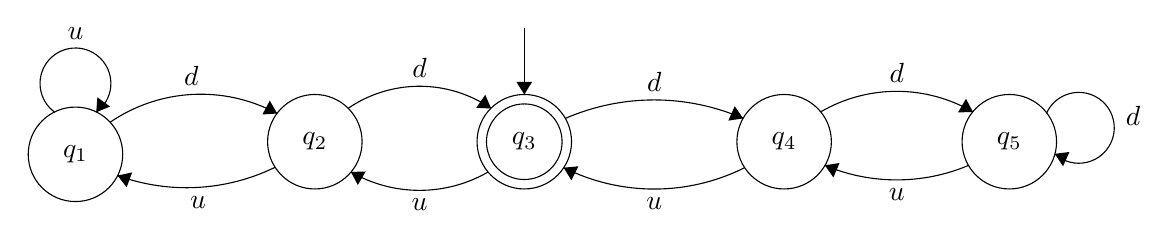
\begin{tikzpicture}[scale=0.2]
\tikzstyle{every node}+=[inner sep=0pt]
\draw [black] (8.3,-10.1) circle (3);
\draw (8.3,-10.1) node {$q_1$};
\draw [black] (23.5,-9.3) circle (3);
\draw (23.5,-9.3) node {$q_2$};
\draw [black] (36.8,-9.3) circle (3);
\draw (36.8,-9.3) node {$q_3$};
\draw [black] (36.8,-9.3) circle (2.4);
\draw [black] (53.3,-9.3) circle (3);
\draw (53.3,-9.3) node {$q_4$};
\draw [black] (67.6,-9.3) circle (3);
\draw (67.6,-9.3) node {$q_5$};
\draw [black] (36.8,-2.1) -- (36.8,-6.3);
\fill [black] (36.8,-6.3) -- (37.3,-5.5) -- (36.3,-5.5);
\draw [black] (6.977,-7.42) arc (234:-54:2.25);
\draw (8.3,-2.85) node [above] {$u$};
\fill [black] (9.62,-7.42) -- (10.5,-7.07) -- (9.69,-6.48);
\draw [black] (10.492,-8.068) arc (124.40866:61.61691:10.202);
\fill [black] (21.11,-7.51) -- (20.64,-6.69) -- (20.17,-7.57);
\draw (15.66,-5.75) node [above] {$d$};
\draw [black] (20.983,-10.92) arc (-63.94561:-110.02881:12.805);
\fill [black] (10.97,-11.45) -- (11.55,-12.19) -- (11.9,-11.25);
\draw (16.09,-12.75) node [below] {$u$};
\draw [black] (25.604,-7.186) arc (124.43892:55.56108:8.038);
\fill [black] (34.7,-7.19) -- (34.32,-6.32) -- (33.75,-7.15);
\draw (30.15,-5.28) node [above] {$d$};
\draw [black] (34.512,-11.217) arc (-59.92561:-120.07439:8.703);
\fill [black] (25.79,-11.22) -- (26.23,-12.05) -- (26.73,-11.19);
\draw (30.15,-12.89) node [below] {$u$};
\draw [black] (39.404,-7.821) arc (113.51604:66.48396:14.15);
\fill [black] (50.7,-7.82) -- (50.16,-7.04) -- (49.76,-7.96);
\draw (45.05,-6.15) node [above] {$d$};
\draw [black] (50.8,-10.945) arc (-63.35828:-116.64172:12.822);
\fill [black] (39.3,-10.95) -- (39.79,-11.75) -- (40.24,-10.86);
\draw (45.05,-12.81) node [below] {$u$};
\draw [black] (55.613,-7.409) arc (120.29559:59.70441:9.588);
\fill [black] (65.29,-7.41) -- (64.85,-6.57) -- (64.34,-7.44);
\draw (60.45,-5.6) node [above] {$d$};
\draw [black] (65.013,-10.803) arc (-67.15252:-112.84748:11.752);
\fill [black] (55.89,-10.8) -- (56.43,-11.57) -- (56.82,-10.65);
\draw (60.45,-12.23) node [below] {$u$};
\draw [black] (69.968,-7.478) arc (155.30993:-132.69007:2.25);
\draw (74.96,-7.66) node [right] {$d$};
\fill [black] (70.49,-10.07) -- (71.01,-10.86) -- (71.42,-9.95);
\end{tikzpicture}
\end{center}
\pagebreak
\problem{1.4}
Each of the following languages is the intersection of two simpler languages. In each part, construct DFAs
for the simpler languages, then combine them using the construction discussed in footnote 3 (page 46) to 
give the state diagram of a DFA for the language given. In all parts, $\sum = \{a,b\}$\\ \\
\problem{1.4 a}
$\{w | w \text{ has at least three a's and at least two b's}\}$\\

1. $\{w | w \text{ has at least three a's}\}$\\
\begin{center}
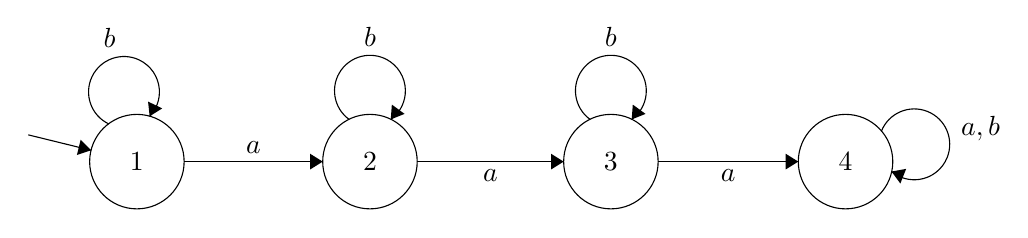
\begin{tikzpicture}[scale=0.2]
\tikzstyle{every node}+=[inner sep=0pt]
\draw [black] (9.1,-9.3) circle (3);
\draw (9.1,-9.3) node {$1$};
\draw [black] (23.9,-9.3) circle (3);
\draw (23.9,-9.3) node {$2$};
\draw [black] (39.2,-9.3) circle (3);
\draw (39.2,-9.3) node {$3$};
\draw [black] (54.1,-9.3) circle (3);
\draw (54.1,-9.3) node {$4$};
\draw [black] (12.1,-9.3) -- (20.9,-9.3);
\fill [black] (20.9,-9.3) -- (20.1,-8.8) -- (20.1,-9.8);
\draw (16.5,-8.8) node [above] {$a$};
\draw [black] (26.9,-9.3) -- (36.2,-9.3);
\fill [black] (36.2,-9.3) -- (35.4,-8.8) -- (35.4,-9.8);
\draw (31.55,-9.8) node [below] {$a$};
\draw [black] (42.2,-9.3) -- (51.1,-9.3);
\fill [black] (51.1,-9.3) -- (50.3,-8.8) -- (50.3,-9.8);
\draw (46.65,-9.8) node [below] {$a$};
\draw [black] (56.377,-7.364) arc (158.10808:-129.89192:2.25);
\draw (61.41,-7.19) node [right] {$a,b$};
\fill [black] (57.02,-9.93) -- (57.58,-10.69) -- (57.95,-9.76);
\draw [black] (37.877,-6.62) arc (234:-54:2.25);
\draw (39.2,-2.05) node [above] {$b$};
\fill [black] (40.52,-6.62) -- (41.4,-6.27) -- (40.59,-5.68);
\draw [black] (22.577,-6.62) arc (234:-54:2.25);
\draw (23.9,-2.05) node [above] {$b$};
\fill [black] (25.22,-6.62) -- (26.1,-6.27) -- (25.29,-5.68);
\draw [black] (7.312,-6.906) arc (244.49148:-43.50852:2.25);
\draw (7.36,-2.07) node [above] {$b$};
\fill [black] (9.91,-6.42) -- (10.71,-5.92) -- (9.81,-5.49);
\draw [black] (2.2,-7.6) -- (6.19,-8.58);
\fill [black] (6.19,-8.58) -- (5.53,-7.91) -- (5.29,-8.88);
\end{tikzpicture}
\end{center}
\vspace{0.5cm}
2. $\{w | w \text{ has at least two b's}\}$\\
\begin{center}
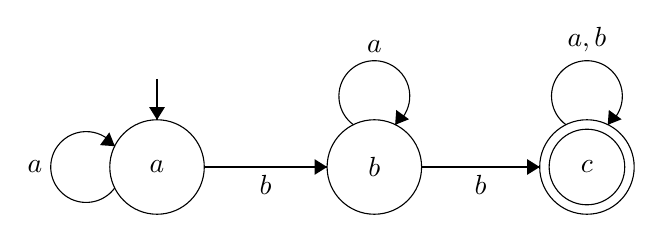
\begin{tikzpicture}[scale=0.2]
\tikzstyle{every node}+=[inner sep=0pt]
\draw [black] (11.8,-10.1) circle (3);
\draw (11.8,-10.1) node {$a$};
\draw [black] (25.6,-10.1) circle (3);
\draw (25.6,-10.1) node {$b$};
\draw [black] (39.1,-10.1) circle (3);
\draw (39.1,-10.1) node {$c$};
\draw [black] (39.1,-10.1) circle (2.4);
\draw [black] (11.8,-4.5) -- (11.8,-7.1);
\fill [black] (11.8,-7.1) -- (12.3,-6.3) -- (11.3,-6.3);
\draw [black] (14.8,-10.1) -- (22.6,-10.1);
\fill [black] (22.6,-10.1) -- (21.8,-9.6) -- (21.8,-10.6);
\draw (18.7,-10.6) node [below] {$b$};
\draw [black] (28.6,-10.1) -- (36.1,-10.1);
\fill [black] (36.1,-10.1) -- (35.3,-9.6) -- (35.3,-10.6);
\draw (32.35,-10.6) node [below] {$b$};
\draw [black] (37.777,-7.42) arc (234:-54:2.25);
\draw (39.1,-2.85) node [above] {$a,b$};
\fill [black] (40.42,-7.42) -- (41.3,-7.07) -- (40.49,-6.48);
\draw [black] (9.12,-11.423) arc (324:36:2.25);
\draw (4.55,-10.1) node [left] {$a$};
\fill [black] (9.12,-8.78) -- (8.77,-7.9) -- (8.18,-8.71);
\draw [black] (24.277,-7.42) arc (234:-54:2.25);
\draw (25.6,-2.85) node [above] {$a$};
\fill [black] (26.92,-7.42) -- (27.8,-7.07) -- (26.99,-6.48);
\end{tikzpicture}
\end{center}

3.$\{w | w \text{ has at least three a's and at least two b's}\}$\\
\begin{center}
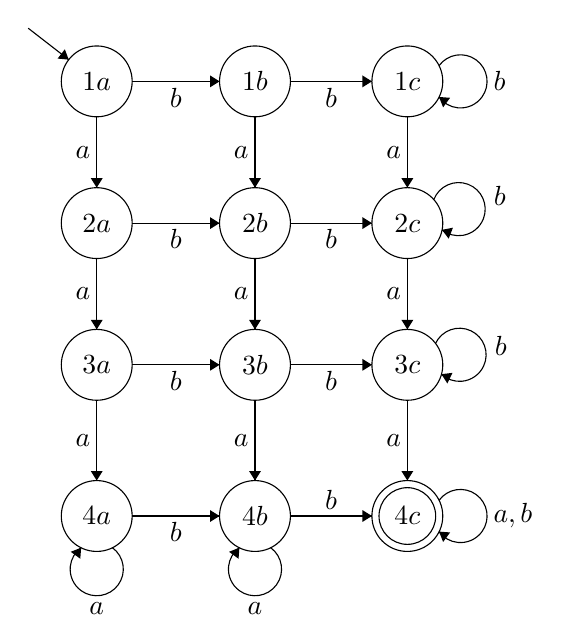
\begin{tikzpicture}[scale=0.15]
\tikzstyle{every node}+=[inner sep=0pt]
\draw [black] (7.4,-5.7) circle (3);
\draw (7.4,-5.7) node {$1a$};
\draw [black] (20.8,-5.7) circle (3);
\draw (20.8,-5.7) node {$1b$};
\draw [black] (33.7,-5.7) circle (3);
\draw (33.7,-5.7) node {$1c$};
\draw [black] (7.4,-17.7) circle (3);
\draw (7.4,-17.7) node {$2a$};
\draw [black] (20.8,-17.7) circle (3);
\draw (20.8,-17.7) node {$2b$};
\draw [black] (33.7,-17.7) circle (3);
\draw (33.7,-17.7) node {$2c$};
\draw [black] (7.4,-29.7) circle (3);
\draw (7.4,-29.7) node {$3a$};
\draw [black] (20.8,-29.7) circle (3);
\draw (20.8,-29.7) node {$3b$};
\draw [black] (33.7,-29.7) circle (3);
\draw (33.7,-29.7) node {$3c$};
\draw [black] (20.8,-42.5) circle (3);
\draw (20.8,-42.5) node {$4b$};
\draw [black] (7.4,-42.5) circle (3);
\draw (7.4,-42.5) node {$4a$};
\draw [black] (33.7,-42.5) circle (3);
\draw (33.7,-42.5) node {$4c$};
\draw [black] (33.7,-42.5) circle (2.4);
\draw [black] (1.6,-1.2) -- (5.03,-3.86);
\fill [black] (5.03,-3.86) -- (4.7,-2.98) -- (4.09,-3.77);
\draw [black] (10.4,-5.7) -- (17.8,-5.7);
\fill [black] (17.8,-5.7) -- (17,-5.2) -- (17,-6.2);
\draw (14.1,-6.2) node [below] {$b$};
\draw [black] (23.8,-5.7) -- (30.7,-5.7);
\fill [black] (30.7,-5.7) -- (29.9,-5.2) -- (29.9,-6.2);
\draw (27.25,-6.2) node [below] {$b$};
\draw [black] (7.4,-8.7) -- (7.4,-14.7);
\fill [black] (7.4,-14.7) -- (7.9,-13.9) -- (6.9,-13.9);
\draw (6.9,-11.7) node [left] {$a$};
\draw [black] (10.4,-17.7) -- (17.8,-17.7);
\fill [black] (17.8,-17.7) -- (17,-17.2) -- (17,-18.2);
\draw (14.1,-18.2) node [below] {$b$};
\draw [black] (20.8,-8.7) -- (20.8,-14.7);
\fill [black] (20.8,-14.7) -- (21.3,-13.9) -- (20.3,-13.9);
\draw (20.3,-11.7) node [left] {$a$};
\draw [black] (23.8,-17.7) -- (30.7,-17.7);
\fill [black] (30.7,-17.7) -- (29.9,-17.2) -- (29.9,-18.2);
\draw (27.25,-18.2) node [below] {$b$};
\draw [black] (33.7,-8.7) -- (33.7,-14.7);
\fill [black] (33.7,-14.7) -- (34.2,-13.9) -- (33.2,-13.9);
\draw (33.2,-11.7) node [left] {$a$};
\draw [black] (7.4,-20.7) -- (7.4,-26.7);
\fill [black] (7.4,-26.7) -- (7.9,-25.9) -- (6.9,-25.9);
\draw (6.9,-23.7) node [left] {$a$};
\draw [black] (20.8,-20.7) -- (20.8,-26.7);
\fill [black] (20.8,-26.7) -- (21.3,-25.9) -- (20.3,-25.9);
\draw (20.3,-23.7) node [left] {$a$};
\draw [black] (33.7,-20.7) -- (33.7,-26.7);
\fill [black] (33.7,-26.7) -- (34.2,-25.9) -- (33.2,-25.9);
\draw (33.2,-23.7) node [left] {$a$};
\draw [black] (10.4,-29.7) -- (17.8,-29.7);
\fill [black] (17.8,-29.7) -- (17,-29.2) -- (17,-30.2);
\draw (14.1,-30.2) node [below] {$b$};
\draw [black] (23.8,-29.7) -- (30.7,-29.7);
\fill [black] (30.7,-29.7) -- (29.9,-29.2) -- (29.9,-30.2);
\draw (27.25,-30.2) node [below] {$b$};
\draw [black] (20.8,-32.7) -- (20.8,-39.5);
\fill [black] (20.8,-39.5) -- (21.3,-38.7) -- (20.3,-38.7);
\draw (20.3,-36.1) node [left] {$a$};
\draw [black] (36.082,-27.895) arc (154.88553:-133.11447:2.25);
\draw (41.06,-28.13) node [right] {$b$};
\fill [black] (36.58,-30.49) -- (37.09,-31.28) -- (37.52,-30.38);
\draw [black] (22.123,-45.18) arc (54:-234:2.25);
\draw (20.8,-49.75) node [below] {$a$};
\fill [black] (19.48,-45.18) -- (18.6,-45.53) -- (19.41,-46.12);
\draw [black] (36.38,-4.377) arc (144:-144:2.25);
\draw (40.95,-5.7) node [right] {$b$};
\fill [black] (36.38,-7.02) -- (36.73,-7.9) -- (37.32,-7.09);
\draw [black] (35.937,-15.719) arc (159.25512:-128.74488:2.25);
\draw (40.98,-15.4) node [right] {$b$};
\fill [black] (36.63,-18.27) -- (37.2,-19.02) -- (37.56,-18.09);
\draw [black] (7.4,-32.7) -- (7.4,-39.5);
\fill [black] (7.4,-39.5) -- (7.9,-38.7) -- (6.9,-38.7);
\draw (6.9,-36.1) node [left] {$a$};
\draw [black] (10.4,-42.5) -- (17.8,-42.5);
\fill [black] (17.8,-42.5) -- (17,-42) -- (17,-43);
\draw (14.1,-43) node [below] {$b$};
\draw [black] (23.8,-42.5) -- (30.7,-42.5);
\fill [black] (30.7,-42.5) -- (29.9,-42) -- (29.9,-43);
\draw (27.25,-42) node [above] {$b$};
\draw [black] (33.7,-32.7) -- (33.7,-39.5);
\fill [black] (33.7,-39.5) -- (34.2,-38.7) -- (33.2,-38.7);
\draw (33.2,-36.1) node [left] {$a$};
\draw [black] (36.38,-41.177) arc (144:-144:2.25);
\draw (40.95,-42.5) node [right] {$a,b$};
\fill [black] (36.38,-43.82) -- (36.73,-44.7) -- (37.32,-43.89);
\draw [black] (8.723,-45.18) arc (54:-234:2.25);
\draw (7.4,-49.75) node [below] {$a$};
\fill [black] (6.08,-45.18) -- (5.2,-45.53) -- (6.01,-46.12);
\end{tikzpicture}
\end{center}


\problem{1.4 c} \\
$\{w | w \text{ has an even number of a's and one ore two b's}\}$\\


1. $\{w | w \text{ has an even number of a's}\}$ \hspace{1cm} 2. $\{w | w \text{ has one or two b's}\}$
\begin{center}
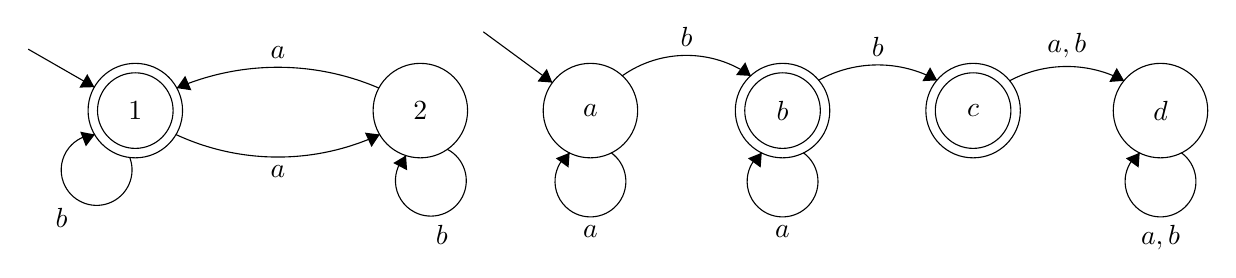
\begin{tikzpicture}[scale=0.2]
\tikzstyle{every node}+=[inner sep=0pt]
\draw [black] (10.1,-7.1) circle (3);
\draw (10.1,-7.1) node {$1$};
\draw [black] (10.1,-7.1) circle (2.4);
\draw [black] (28.2,-7.1) circle (3);
\draw (28.2,-7.1) node {$2$};
\draw [black] (39,-7.1) circle (3);
\draw (39,-7.1) node {$a$};
\draw [black] (51.2,-7.1) circle (3);
\draw (51.2,-7.1) node {$b$};
\draw [black] (51.2,-7.1) circle (2.4);
\draw [black] (63.3,-7.1) circle (3);
\draw (63.3,-7.1) node {$c$};
\draw [black] (63.3,-7.1) circle (2.4);
\draw [black] (75.2,-7.1) circle (3);
\draw (75.2,-7.1) node {$d$};
\draw [black] (3.3,-3.2) -- (7.5,-5.61);
\fill [black] (7.5,-5.61) -- (7.05,-4.78) -- (6.55,-5.64);
\draw [black] (25.62,-8.621) arc (-65.08079:-114.91921:15.355);
\fill [black] (25.62,-8.62) -- (24.68,-8.5) -- (25.1,-9.41);
\draw (19.15,-10.55) node [below] {$a$};
\draw [black] (12.732,-5.669) arc (113.25012:66.74988:16.259);
\fill [black] (12.73,-5.67) -- (13.66,-5.81) -- (13.27,-4.89);
\draw (19.15,-3.85) node [above] {$a$};
\draw [black] (32.2,-2.1) -- (36.58,-5.32);
\fill [black] (36.58,-5.32) -- (36.23,-4.45) -- (35.64,-5.25);
\draw [black] (41.007,-4.901) arc (125.43267:54.56733:7.059);
\fill [black] (49.19,-4.9) -- (48.83,-4.03) -- (48.25,-4.84);
\draw (45.1,-3.09) node [above] {$b$};
\draw [black] (53.479,-5.177) arc (119.07851:60.92149:7.76);
\fill [black] (61.02,-5.18) -- (60.57,-4.35) -- (60.08,-5.23);
\draw (57.25,-3.7) node [above] {$b$};
\draw [black] (65.607,-5.212) arc (118.16267:61.83733:7.719);
\fill [black] (72.89,-5.21) -- (72.42,-4.39) -- (71.95,-5.28);
\draw (69.25,-3.8) node [above] {$a,b$};
\draw [black] (40.323,-9.78) arc (54:-234:2.25);
\draw (39,-14.35) node [below] {$a$};
\fill [black] (37.68,-9.78) -- (36.8,-10.13) -- (37.61,-10.72);
\draw [black] (52.523,-9.78) arc (54:-234:2.25);
\draw (51.2,-14.35) node [below] {$a$};
\fill [black] (49.88,-9.78) -- (49,-10.13) -- (49.81,-10.72);
\draw [black] (76.523,-9.78) arc (54:-234:2.25);
\draw (75.2,-14.35) node [below] {$a,b$};
\fill [black] (73.88,-9.78) -- (73,-10.13) -- (73.81,-10.72);
\draw [black] (9.744,-10.067) arc (20.88866:-267.11134:2.25);
\draw (5.41,-13.25) node [below] {$b$};
\fill [black] (7.53,-8.62) -- (6.6,-8.44) -- (6.96,-9.37);
\draw [black] (29.905,-9.554) arc (62.53077:-225.46923:2.25);
\draw (29.57,-14.37) node [below] {$b$};
\fill [black] (27.29,-9.95) -- (26.48,-10.43) -- (27.36,-10.89);
\end{tikzpicture}
\end{center}

3. $\{w | w \text{ has an even number of a's and one ore two b's}\}$\\
\begin{center}
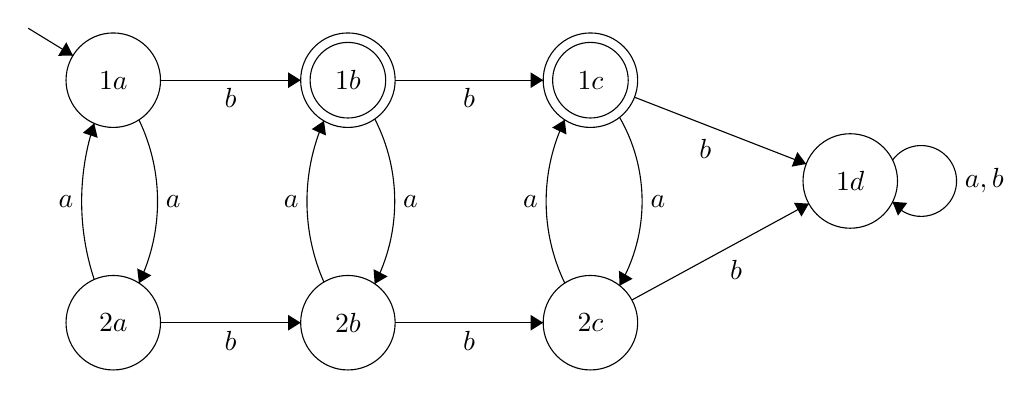
\begin{tikzpicture}[scale=0.2]
\tikzstyle{every node}+=[inner sep=0pt]
\draw [black] (8.1,-6.6) circle (3);
\draw (8.1,-6.6) node {$1a$};
\draw [black] (8.1,-22) circle (3);
\draw (8.1,-22) node {$2a$};
\draw [black] (23,-6.6) circle (3);
\draw (23,-6.6) node {$1b$};
\draw [black] (23,-6.6) circle (2.4);
\draw [black] (23,-22) circle (3);
\draw (23,-22) node {$2b$};
\draw [black] (38.4,-6.6) circle (3);
\draw (38.4,-6.6) node {$1c$};
\draw [black] (38.4,-6.6) circle (2.4);
\draw [black] (38.4,-22) circle (3);
\draw (38.4,-22) node {$2c$};
\draw [black] (54.9,-13) circle (3);
\draw (54.9,-13) node {$1d$};
\draw [black] (2.7,-3.3) -- (5.54,-5.04);
\fill [black] (5.54,-5.04) -- (5.12,-4.19) -- (4.6,-5.05);
\draw [black] (9.727,-9.111) arc (25.73953:-25.73953:11.948);
\fill [black] (9.73,-19.49) -- (10.52,-18.99) -- (9.62,-18.55);
\draw (11.41,-14.3) node [right] {$a$};
\draw [black] (24.704,-9.058) arc (27.23117:-27.23117:11.455);
\fill [black] (24.7,-19.54) -- (25.52,-19.06) -- (24.63,-18.6);
\draw (26.47,-14.3) node [right] {$a$};
\draw [black] (40.246,-8.952) arc (30.0658:-30.0658:10.674);
\fill [black] (40.25,-19.65) -- (41.08,-19.21) -- (40.21,-18.7);
\draw (42.18,-14.3) node [right] {$a$};
\draw [black] (6.892,-19.259) arc (-161.66604:-198.33396:15.765);
\fill [black] (6.89,-9.34) -- (6.17,-9.94) -- (7.11,-10.26);
\draw (5.59,-14.3) node [left] {$a$};
\draw [black] (21.478,-19.423) arc (-156.21298:-203.78702:12.7);
\fill [black] (21.48,-9.18) -- (20.7,-9.71) -- (21.61,-10.11);
\draw (19.9,-14.3) node [left] {$a$};
\draw [black] (36.773,-19.489) arc (-154.24867:-205.75133:11.944);
\fill [black] (36.77,-9.11) -- (35.97,-9.61) -- (36.88,-10.05);
\draw (35.09,-14.3) node [left] {$a$};
\draw [black] (11.1,-6.6) -- (20,-6.6);
\fill [black] (20,-6.6) -- (19.2,-6.1) -- (19.2,-7.1);
\draw (15.55,-7.1) node [below] {$b$};
\draw [black] (11.1,-22) -- (20,-22);
\fill [black] (20,-22) -- (19.2,-21.5) -- (19.2,-22.5);
\draw (15.55,-22.5) node [below] {$b$};
\draw [black] (26,-6.6) -- (35.4,-6.6);
\fill [black] (35.4,-6.6) -- (34.6,-6.1) -- (34.6,-7.1);
\draw (30.7,-7.1) node [below] {$b$};
\draw [black] (26,-22) -- (35.4,-22);
\fill [black] (35.4,-22) -- (34.6,-21.5) -- (34.6,-22.5);
\draw (30.7,-22.5) node [below] {$b$};
\draw [black] (41.2,-7.68) -- (52.1,-11.92);
\fill [black] (52.1,-11.92) -- (51.54,-11.16) -- (51.18,-12.09);
\draw (45.7,-10.32) node [below] {$b$};
\draw [black] (41.03,-20.56) -- (52.27,-14.44);
\fill [black] (52.27,-14.44) -- (51.32,-14.38) -- (51.8,-15.26);
\draw (47.65,-18) node [below] {$b$};
\draw [black] (57.58,-11.677) arc (144:-144:2.25);
\draw (62.15,-13) node [right] {$a,b$};
\fill [black] (57.58,-14.32) -- (57.93,-15.2) -- (58.52,-14.39);
\end{tikzpicture}
\end{center}
\vspace{1cm}
\problem{1.6}
Give state diagrams of DFAs recognizing the following languages. In all parts, 
the alphabet is $\{0,1\}$\\ \\
\problem{1.6 f}
$\{w|w \text{ doesn't contain the substring } 110\}$
\begin{center}
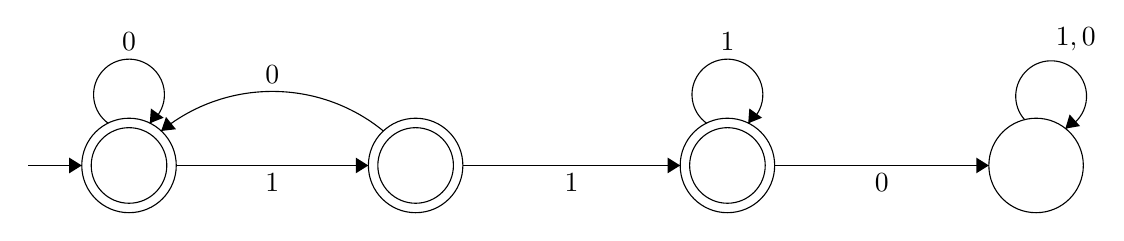
\begin{tikzpicture}[scale=0.2]
\tikzstyle{every node}+=[inner sep=0pt]
\draw [black] (10.6,-11.7) circle (3);
\draw [black] (10.6,-11.7) circle (2.4);
\draw [black] (28.8,-11.7) circle (3);
\draw [black] (28.8,-11.7) circle (2.4);
\draw [black] (48.6,-11.7) circle (3);
\draw [black] (48.6,-11.7) circle (2.4);
\draw [black] (68.2,-11.7) circle (3);
\draw [black] (4.2,-11.7) -- (7.6,-11.7);
\fill [black] (7.6,-11.7) -- (6.8,-11.2) -- (6.8,-12.2);
\draw [black] (13.6,-11.7) -- (25.8,-11.7);
\fill [black] (25.8,-11.7) -- (25,-11.2) -- (25,-12.2);
\draw (19.7,-12.2) node [below] {$1$};
\draw [black] (31.8,-11.7) -- (45.6,-11.7);
\fill [black] (45.6,-11.7) -- (44.8,-11.2) -- (44.8,-12.2);
\draw (38.7,-12.2) node [below] {$1$};
\draw [black] (51.6,-11.7) -- (65.2,-11.7);
\fill [black] (65.2,-11.7) -- (64.4,-11.2) -- (64.4,-12.2);
\draw (58.4,-12.2) node [below] {$0$};
\draw [black] (9.277,-9.02) arc (234:-54:2.25);
\draw (10.6,-4.45) node [above] {$0$};
\fill [black] (11.92,-9.02) -- (12.8,-8.67) -- (11.99,-8.08);
\draw [black] (12.642,-9.514) arc (129.24296:50.75704:11.157);
\fill [black] (12.64,-9.51) -- (13.58,-9.4) -- (12.95,-8.62);
\draw (19.7,-6.5) node [above] {$0$};
\draw [black] (67.477,-8.801) arc (221.73523:-66.26477:2.25);
\draw (70.72,-4.46) node [above] {$1,0$};
\fill [black] (70.06,-9.36) -- (70.99,-9.2) -- (70.33,-8.46);
\draw [black] (47.277,-9.02) arc (234:-54:2.25);
\draw (48.6,-4.45) node [above] {$1$};
\fill [black] (49.92,-9.02) -- (50.8,-8.67) -- (49.99,-8.08);
\end{tikzpicture}
\end{center}

\pagebreak

\problem{1.6 l}

$\{w|w \text{ contains an even number os 0s, or contains exactly two 1s }\}$\\

1. $\{w|w \text{ contains an even number os 0s}\}$\\
\begin{center}
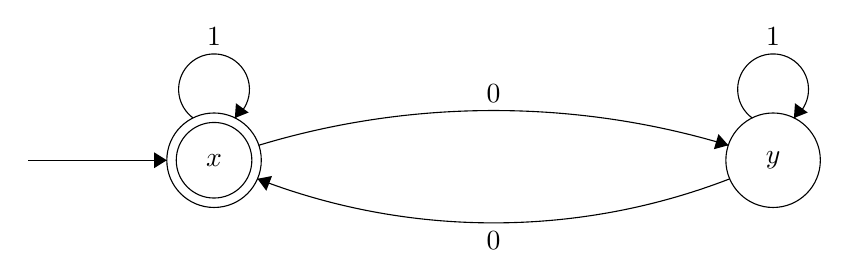
\begin{tikzpicture}[scale=0.2]
\tikzstyle{every node}+=[inner sep=0pt]
\draw [black] (14.8,-9.9) circle (3);
\draw (14.8,-9.9) node {$x$};
\draw [black] (14.8,-9.9) circle (2.4);
\draw [black] (50.3,-9.9) circle (3);
\draw (50.3,-9.9) node {$y$};
\draw [black] (3,-9.9) -- (11.8,-9.9);
\fill [black] (11.8,-9.9) -- (11,-9.4) -- (11,-10.4);
\draw [black] (17.645,-8.948) arc (106.83285:73.16715:51.473);
\fill [black] (47.46,-8.95) -- (46.83,-8.24) -- (46.54,-9.2);
\draw (32.55,-6.24) node [above] {$0$};
\draw [black] (47.543,-11.082) arc (-68.8638:-111.1362:41.58);
\fill [black] (17.56,-11.08) -- (18.12,-11.84) -- (18.48,-10.9);
\draw (32.55,-14.38) node [below] {$0$};
\draw [black] (13.477,-7.22) arc (234:-54:2.25);
\draw (14.8,-2.65) node [above] {$1$};
\fill [black] (16.12,-7.22) -- (17,-6.87) -- (16.19,-6.28);
\draw [black] (48.977,-7.22) arc (234:-54:2.25);
\draw (50.3,-2.65) node [above] {$1$};
\fill [black] (51.62,-7.22) -- (52.5,-6.87) -- (51.69,-6.28);
\end{tikzpicture}
\end{center}

2. $\{w|w \text{ contains exactly two 1s }\}$\\
\begin{center}
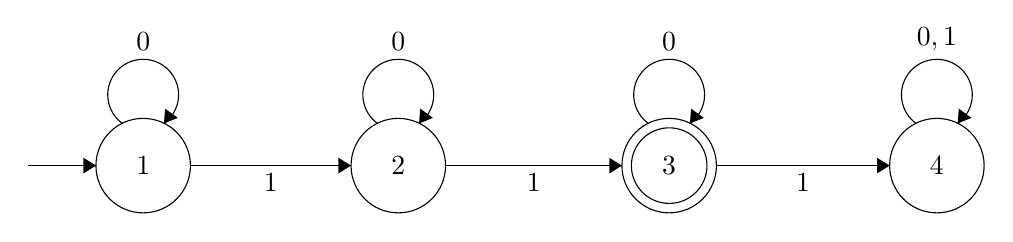
\begin{tikzpicture}[scale=0.2]
\tikzstyle{every node}+=[inner sep=0pt]
\draw [black] (9.1,-9.3) circle (3);
\draw (9.1,-9.3) node {$1$};
\draw [black] (25.3,-9.3) circle (3);
\draw (25.3,-9.3) node {$2$};
\draw [black] (42.5,-9.3) circle (3);
\draw (42.5,-9.3) node {$3$};
\draw [black] (42.5,-9.3) circle (2.4);
\draw [black] (59.5,-9.3) circle (3);
\draw (59.5,-9.3) node {$4$};
\draw [black] (1.8,-9.3) -- (6.1,-9.3);
\fill [black] (6.1,-9.3) -- (5.3,-8.8) -- (5.3,-9.8);
\draw [black] (12.1,-9.3) -- (22.3,-9.3);
\fill [black] (22.3,-9.3) -- (21.5,-8.8) -- (21.5,-9.8);
\draw (17.2,-9.8) node [below] {$1$};
\draw [black] (28.3,-9.3) -- (39.5,-9.3);
\fill [black] (39.5,-9.3) -- (38.7,-8.8) -- (38.7,-9.8);
\draw (33.9,-9.8) node [below] {$1$};
\draw [black] (45.5,-9.3) -- (56.5,-9.3);
\fill [black] (56.5,-9.3) -- (55.7,-8.8) -- (55.7,-9.8);
\draw (51,-9.8) node [below] {$1$};
\draw [black] (58.177,-6.62) arc (234:-54:2.25);
\draw (59.5,-2.05) node [above] {$0,1$};
\fill [black] (60.82,-6.62) -- (61.7,-6.27) -- (60.89,-5.68);
\draw [black] (41.177,-6.62) arc (234:-54:2.25);
\draw (42.5,-2.05) node [above] {$0$};
\fill [black] (43.82,-6.62) -- (44.7,-6.27) -- (43.89,-5.68);
\draw [black] (23.977,-6.62) arc (234:-54:2.25);
\draw (25.3,-2.05) node [above] {$0$};
\fill [black] (26.62,-6.62) -- (27.5,-6.27) -- (26.69,-5.68);
\draw [black] (7.777,-6.62) arc (234:-54:2.25);
\draw (9.1,-2.05) node [above] {$0$};
\fill [black] (10.42,-6.62) -- (11.3,-6.27) -- (10.49,-5.68);
\end{tikzpicture}
\end{center}

3. $\{w|w \text{ contains an even number os 0s, or contains exactly two 1s }\}$\\
\begin{center}
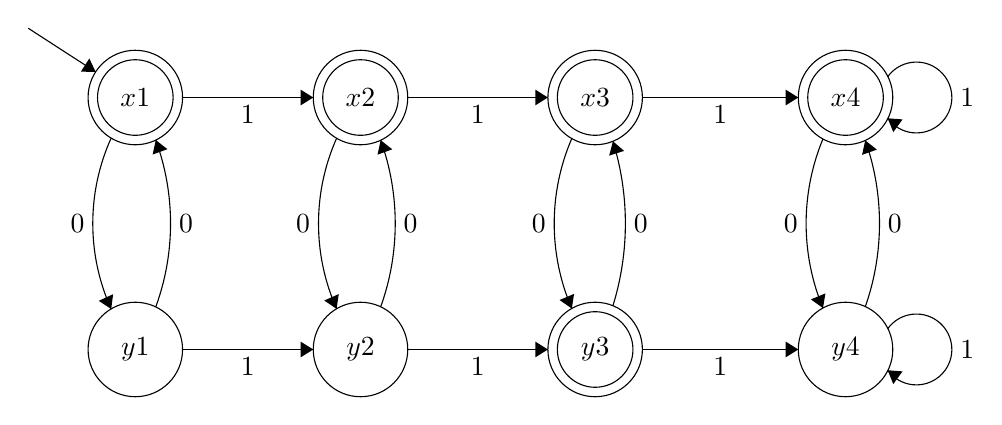
\begin{tikzpicture}[scale=0.2]
\tikzstyle{every node}+=[inner sep=0pt]
\draw [black] (8.6,-5.7) circle (3);
\draw [black] (8.6,-5.7) circle (2.4);
\draw (8.6,-5.7) node {$x1$};
\draw [black] (22.9,-5.7) circle (3);
\draw [black] (22.9,-5.7) circle (2.4);
\draw (22.9,-5.7) node {$x2$};
\draw [black] (37.8,-5.7) circle (3);
\draw (37.8,-5.7) node {$x3$};
\draw [black] (37.8,-5.7) circle (2.4);
\draw [black] (53.7,-5.7) circle (3);
\draw [black] (53.7,-5.7) circle (2.4);
\draw (53.7,-5.7) node {$x4$};
\draw [black] (8.6,-21.7) circle (3);
\draw (8.6,-21.7) node {$y1$};
\draw [black] (22.9,-21.7) circle (3);
\draw (22.9,-21.7) node {$y2$};
\draw [black] (37.8,-21.7) circle (3);
\draw [black] (37.8,-21.7) circle (2.4);
\draw (37.8,-21.7) node {$y3$};
\draw [black] (53.7,-21.7) circle (3);
\draw (53.7,-21.7) node {$y4$};
\draw [black] (1.8,-1.3) -- (6.08,-4.07);
\fill [black] (6.08,-4.07) -- (5.68,-3.22) -- (5.14,-4.06);
\draw [black] (7.067,-19.129) arc (-155.70648:-204.29352:13.196);
\fill [black] (7.07,-19.13) -- (7.19,-18.19) -- (6.28,-18.61);
\draw (5.4,-13.7) node [left] {$0$};
\draw [black] (11.6,-5.7) -- (19.9,-5.7);
\fill [black] (19.9,-5.7) -- (19.1,-5.2) -- (19.1,-6.2);
\draw (15.75,-6.2) node [below] {$1$};
\draw [black] (9.898,-8.4) arc (20.1002:-20.1002:15.423);
\fill [black] (9.9,-8.4) -- (9.7,-9.32) -- (10.64,-8.98);
\draw (11.34,-13.7) node [right] {$0$};
\draw [black] (11.6,-21.7) -- (19.9,-21.7);
\fill [black] (19.9,-21.7) -- (19.1,-21.2) -- (19.1,-22.2);
\draw (15.75,-22.2) node [below] {$1$};
\draw [black] (21.384,-19.119) arc (-156.02011:-203.97989:13.333);
\fill [black] (21.38,-19.12) -- (21.52,-18.18) -- (20.6,-18.59);
\draw (19.73,-13.7) node [left] {$0$};
\draw [black] (24.181,-8.408) arc (19.81475:-19.81475:15.613);
\fill [black] (24.18,-8.41) -- (23.98,-9.33) -- (24.92,-8.99);
\draw (25.61,-13.7) node [right] {$0$};
\draw [black] (25.9,-5.7) -- (34.8,-5.7);
\fill [black] (34.8,-5.7) -- (34,-5.2) -- (34,-6.2);
\draw (30.35,-6.2) node [below] {$1$};
\draw [black] (25.9,-21.7) -- (34.8,-21.7);
\fill [black] (34.8,-21.7) -- (34,-21.2) -- (34,-22.2);
\draw (30.35,-22.2) node [below] {$1$};
\draw [black] (36.317,-19.099) arc (-156.62331:-203.37669:13.608);
\fill [black] (36.32,-19.1) -- (36.46,-18.17) -- (35.54,-18.56);
\draw (34.7,-13.7) node [left] {$0$};
\draw [black] (38.928,-8.476) arc (17.2318:-17.2318:17.634);
\fill [black] (38.93,-8.48) -- (38.69,-9.39) -- (39.64,-9.09);
\draw (40.22,-13.7) node [right] {$0$};
\draw [black] (40.8,-5.7) -- (50.7,-5.7);
\fill [black] (50.7,-5.7) -- (49.9,-5.2) -- (49.9,-6.2);
\draw (45.75,-6.2) node [below] {$1$};
\draw [black] (40.8,-21.7) -- (50.7,-21.7);
\fill [black] (50.7,-21.7) -- (49.9,-21.2) -- (49.9,-22.2);
\draw (45.75,-22.2) node [below] {$1$};
\draw [black] (52.265,-19.072) arc (-157.49547:-202.50453:14.034);
\fill [black] (52.27,-19.07) -- (52.42,-18.14) -- (51.5,-18.52);
\draw (50.7,-13.7) node [left] {$0$};
\draw [black] (54.955,-8.42) arc (19.36837:-19.36837:15.921);
\fill [black] (54.95,-8.42) -- (54.75,-9.34) -- (55.69,-9.01);
\draw (56.36,-13.7) node [right] {$0$};
\draw [black] (56.38,-4.377) arc (144:-144:2.25);
\draw (60.95,-5.7) node [right] {$1$};
\fill [black] (56.38,-7.02) -- (56.73,-7.9) -- (57.32,-7.09);
\draw [black] (56.38,-20.377) arc (144:-144:2.25);
\draw (60.95,-21.7) node [right] {$1$};
\fill [black] (56.38,-23.02) -- (56.73,-23.9) -- (57.32,-23.09);
\end{tikzpicture}
\end{center}


\pagebreak

\problem{1.7}
Give state diagrams of NFAs with the specified number of states recognizing each of the following languages. In all parts,
the alphabet is $\{0,1\}$. \\ \\


\problem{1.7 c}
$\{w|w \text{ contains an even number os 0s, or contains exactly two 1s }\}$ With six states.\\
1. $\{w|w \text{ contains an even number os 0s}\}$\\
\begin{center}
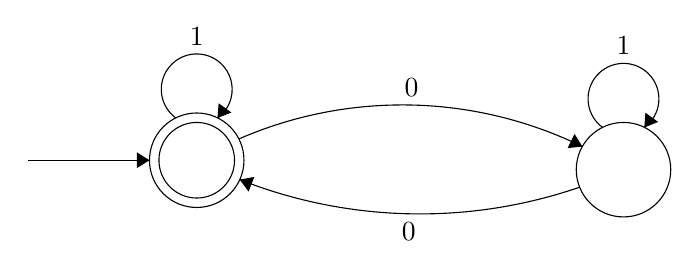
\begin{tikzpicture}[scale=0.2]
\tikzstyle{every node}+=[inner sep=0pt]
\draw [black] (17.1,-11.5) circle (3);
\draw [black] (17.1,-11.5) circle (2.4);
\draw [black] (44.2,-12.1) circle (3);
\draw [black] (6.4,-11.5) -- (14.1,-11.5);
\fill [black] (14.1,-11.5) -- (13.3,-11) -- (13.3,-12);
\draw [black] (19.776,-10.148) arc (113.51064:63.95269:26.026);
\fill [black] (41.59,-10.63) -- (41.09,-9.83) -- (40.65,-10.73);
\draw (30.74,-7.47) node [above] {$0$};
\draw [black] (41.415,-13.212) arc (-70.99514:-111.54152:31.15);
\fill [black] (19.83,-12.73) -- (20.39,-13.49) -- (20.76,-12.56);
\draw (30.57,-15.42) node [below] {$0$};
\draw [black] (15.777,-8.82) arc (234:-54:2.25);
\draw (17.1,-4.25) node [above] {$1$};
\fill [black] (18.42,-8.82) -- (19.3,-8.47) -- (18.49,-7.88);
\draw [black] (42.877,-9.42) arc (234:-54:2.25);
\draw (44.2,-4.85) node [above] {$1$};
\fill [black] (45.52,-9.42) -- (46.4,-9.07) -- (45.59,-8.48);
\end{tikzpicture}
\end{center}

2. $\{w|w \text{ contains exactly two 1s }\}$\\
\begin{center}
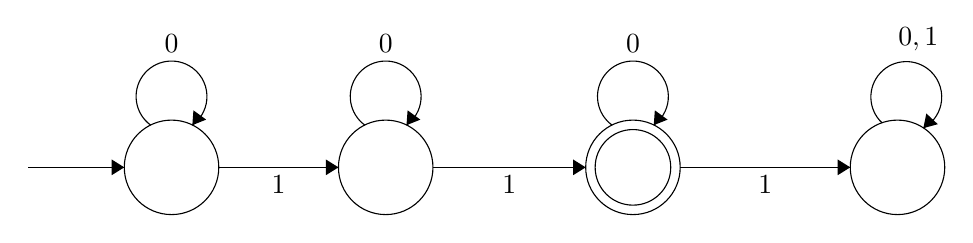
\begin{tikzpicture}[scale=0.2]
\tikzstyle{every node}+=[inner sep=0pt]
\draw [black] (10.5,-10.2) circle (3);
\draw [black] (24.1,-10.2) circle (3);
\draw [black] (39.8,-10.2) circle (3);
\draw [black] (39.8,-10.2) circle (2.4);
\draw [black] (56.6,-10.2) circle (3);
\draw [black] (1.4,-10.2) -- (7.5,-10.2);
\fill [black] (7.5,-10.2) -- (6.7,-9.7) -- (6.7,-10.7);
\draw [black] (13.5,-10.2) -- (21.1,-10.2);
\fill [black] (21.1,-10.2) -- (20.3,-9.7) -- (20.3,-10.7);
\draw (17.3,-10.7) node [below] {$1$};
\draw [black] (27.1,-10.2) -- (36.8,-10.2);
\fill [black] (36.8,-10.2) -- (36,-9.7) -- (36,-10.7);
\draw (31.95,-10.7) node [below] {$1$};
\draw [black] (9.177,-7.52) arc (234:-54:2.25);
\draw (10.5,-2.95) node [above] {$0$};
\fill [black] (11.82,-7.52) -- (12.7,-7.17) -- (11.89,-6.58);
\draw [black] (22.777,-7.52) arc (234:-54:2.25);
\draw (24.1,-2.95) node [above] {$0$};
\fill [black] (25.42,-7.52) -- (26.3,-7.17) -- (25.49,-6.58);
\draw [black] (38.477,-7.52) arc (234:-54:2.25);
\draw (39.8,-2.95) node [above] {$0$};
\fill [black] (41.12,-7.52) -- (42,-7.17) -- (41.19,-6.58);
\draw [black] (42.8,-10.2) -- (53.6,-10.2);
\fill [black] (53.6,-10.2) -- (52.8,-9.7) -- (52.8,-10.7);
\draw (48.2,-10.7) node [below] {$1$};
\draw [black] (55.62,-7.377) arc (226.87498:-61.12502:2.25);
\draw (57.92,-2.84) node [above] {$0,1$};
\fill [black] (58.24,-7.71) -- (59.16,-7.46) -- (58.43,-6.78);
\end{tikzpicture}
\end{center}


3. $\{w|w \text{ contains an even number os 0s, or contains exactly two 1s }\}$\\
\begin{center}
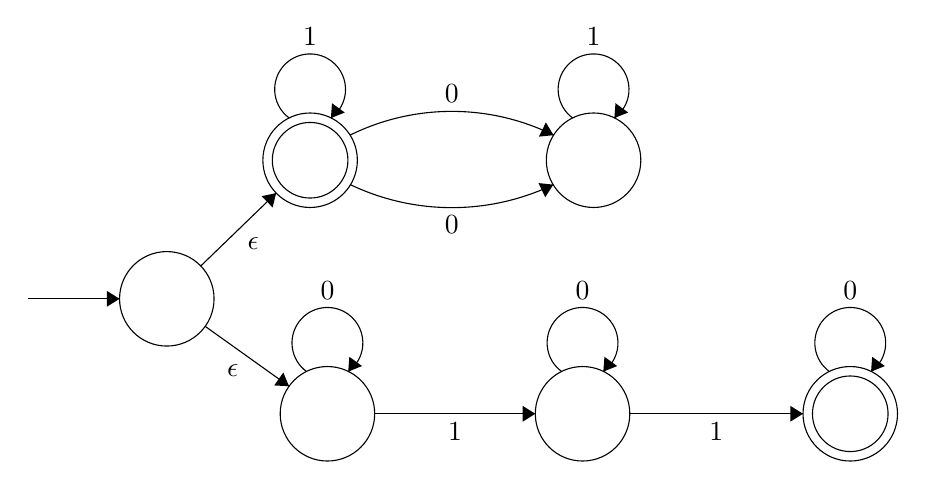
\begin{tikzpicture}[scale=0.2]
\tikzstyle{every node}+=[inner sep=0pt]
\draw [black] (10.1,-18.6) circle (3);
\draw [black] (19.2,-9.8) circle (3);
\draw [black] (19.2,-9.8) circle (2.4);
\draw [black] (37.2,-9.8) circle (3);
\draw [black] (20.3,-25.9) circle (3);
\draw [black] (36.5,-25.9) circle (3);
\draw [black] (53.5,-25.9) circle (3);
\draw [black] (53.5,-25.9) circle (2.4);
\draw [black] (1.3,-18.6) -- (7.1,-18.6);
\fill [black] (7.1,-18.6) -- (6.3,-18.1) -- (6.3,-19.1);
\draw [black] (12.26,-16.51) -- (17.04,-11.89);
\fill [black] (17.04,-11.89) -- (16.12,-12.08) -- (16.82,-12.8);
\draw (15.59,-14.68) node [below] {$\epsilon$};
\draw [black] (12.54,-20.35) -- (17.86,-24.15);
\fill [black] (17.86,-24.15) -- (17.5,-23.28) -- (16.92,-24.1);
\draw (14.28,-22.75) node [below] {$\epsilon$};
\draw [black] (21.735,-8.206) arc (116.27973:63.72027:14.602);
\fill [black] (34.66,-8.21) -- (34.17,-7.4) -- (33.73,-8.3);
\draw (28.2,-6.2) node [above] {$0$};
\draw [black] (34.639,-11.353) arc (-64.50192:-115.49808:14.959);
\fill [black] (34.64,-11.35) -- (33.7,-11.25) -- (34.13,-12.15);
\draw (28.2,-13.31) node [below] {$0$};
\draw [black] (23.3,-25.9) -- (33.5,-25.9);
\fill [black] (33.5,-25.9) -- (32.7,-25.4) -- (32.7,-26.4);
\draw (28.4,-26.4) node [below] {$1$};
\draw [black] (39.5,-25.9) -- (50.5,-25.9);
\fill [black] (50.5,-25.9) -- (49.7,-25.4) -- (49.7,-26.4);
\draw (45,-26.4) node [below] {$1$};
\draw [black] (17.877,-7.12) arc (234:-54:2.25);
\draw (19.2,-2.55) node [above] {$1$};
\fill [black] (20.52,-7.12) -- (21.4,-6.77) -- (20.59,-6.18);
\draw [black] (35.877,-7.12) arc (234:-54:2.25);
\draw (37.2,-2.55) node [above] {$1$};
\fill [black] (38.52,-7.12) -- (39.4,-6.77) -- (38.59,-6.18);
\draw [black] (18.977,-23.22) arc (234:-54:2.25);
\draw (20.3,-18.65) node [above] {$0$};
\fill [black] (21.62,-23.22) -- (22.5,-22.87) -- (21.69,-22.28);
\draw [black] (35.177,-23.22) arc (234:-54:2.25);
\draw (36.5,-18.65) node [above] {$0$};
\fill [black] (37.82,-23.22) -- (38.7,-22.87) -- (37.89,-22.28);
\draw [black] (52.177,-23.22) arc (234:-54:2.25);
\draw (53.5,-18.65) node [above] {$0$};
\fill [black] (54.82,-23.22) -- (55.7,-22.87) -- (54.89,-22.28);
\end{tikzpicture}
\end{center}

\pagebreak

\problem{1.7 e}
The language $0^*1^*0^+$ with three states

\begin{center}
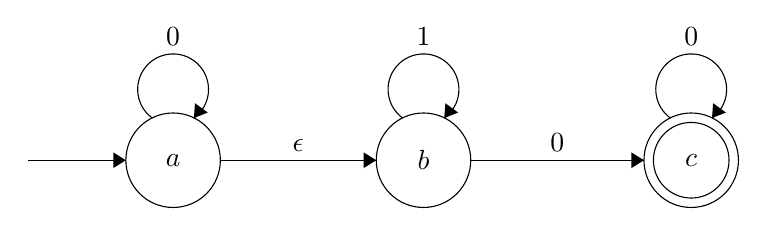
\begin{tikzpicture}[scale=0.2]
\tikzstyle{every node}+=[inner sep=0pt]
\draw [black] (10.6,-10.2) circle (3);
\draw (10.6,-10.2) node {$a$};
\draw [black] (26.5,-10.2) circle (3);
\draw (26.5,-10.2) node {$b$};
\draw [black] (43.5,-10.2) circle (3);
\draw (43.5,-10.2) node {$c$};
\draw [black] (43.5,-10.2) circle (2.4);
\draw [black] (9.277,-7.52) arc (234:-54:2.25);
\draw (10.6,-2.95) node [above] {$0$};
\fill [black] (11.92,-7.52) -- (12.8,-7.17) -- (11.99,-6.58);
\draw [black] (13.6,-10.2) -- (23.5,-10.2);
\fill [black] (23.5,-10.2) -- (22.7,-9.7) -- (22.7,-10.7);
\draw (18.55,-9.7) node [above] {$\epsilon$};
\draw [black] (25.177,-7.52) arc (234:-54:2.25);
\draw (26.5,-2.95) node [above] {$1$};
\fill [black] (27.82,-7.52) -- (28.7,-7.17) -- (27.89,-6.58);
\draw [black] (29.5,-10.2) -- (40.5,-10.2);
\fill [black] (40.5,-10.2) -- (39.7,-9.7) -- (39.7,-10.7);
\draw (35,-9.7) node [above] {$0$};
\draw [black] (42.177,-7.52) arc (234:-54:2.25);
\draw (43.5,-2.95) node [above] {$0$};
\fill [black] (44.82,-7.52) -- (45.7,-7.17) -- (44.89,-6.58);
\draw [black] (1.4,-10.2) -- (7.6,-10.2);
\fill [black] (7.6,-10.2) -- (6.8,-9.7) -- (6.8,-10.7);
\end{tikzpicture}
\end{center}

\vspace{1cm}
\problem{1.12}
Let $D = \{w | w$ contains an even number of a's and an odd number of b's
and does not contain the substring $ab\}$. Give a DFA with five state that recognizes
D and a regular expression that generates D. (Suggestion: Describe D more simply.)\\

We can exclude all strings that starts with a from the DFA, more simply
$D = \{b^{2k}a^{2k+1} \}$.\\
D is recognized by the following DFA:
\begin{center}
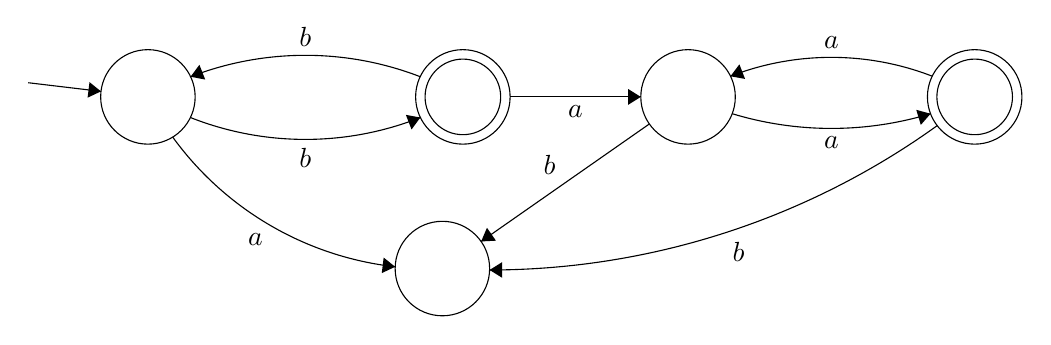
\begin{tikzpicture}[scale=0.2]
\tikzstyle{every node}+=[inner sep=0pt]
\draw [black] (8.3,-6.2) circle (3);
\draw [black] (28.3,-6.2) circle (3);
\draw [black] (28.3,-6.2) circle (2.4);
\draw [black] (27,-17.1) circle (3);
\draw [black] (42.6,-6.2) circle (3);
\draw [black] (60.8,-6.2) circle (3);
\draw [black] (60.8,-6.2) circle (2.4);
\draw [black] (0.7,-5.3) -- (5.32,-5.85);
\fill [black] (5.32,-5.85) -- (4.59,-5.26) -- (4.47,-6.25);
\draw [black] (24.005,-16.987) arc (-96.40192:-144.07284:20.237);
\fill [black] (24,-16.99) -- (23.27,-16.4) -- (23.15,-17.39);
\draw (15.13,-14.86) node [below] {$a$};
\draw [black] (25.604,-7.509) arc (-68.43209:-111.56791:19.869);
\fill [black] (25.6,-7.51) -- (24.68,-7.34) -- (25.04,-8.27);
\draw (18.3,-9.4) node [below] {$b$};
\draw [black] (11.009,-4.917) arc (111.10518:68.89482:20.249);
\fill [black] (11.01,-4.92) -- (11.94,-5.1) -- (11.57,-4.16);
\draw (18.3,-3.06) node [above] {$b$};
\draw [black] (31.3,-6.2) -- (39.6,-6.2);
\fill [black] (39.6,-6.2) -- (38.8,-5.7) -- (38.8,-6.7);
\draw (35.45,-6.7) node [below] {$a$};
\draw [black] (40.14,-7.92) -- (29.46,-15.38);
\fill [black] (29.46,-15.38) -- (30.4,-15.33) -- (29.83,-14.51);
\draw (33.8,-11.15) node [above] {$b$};
\draw [black] (57.999,-7.267) arc (-73.11305:-106.88695:21.683);
\fill [black] (58,-7.27) -- (57.09,-7.02) -- (57.38,-7.98);
\draw (51.7,-8.7) node [below] {$a$};
\draw [black] (45.293,-4.886) arc (111.16929:68.83071:17.742);
\fill [black] (45.29,-4.89) -- (46.22,-5.06) -- (45.86,-4.13);
\draw (51.7,-3.19) node [above] {$a$};
\draw [black] (58.42,-8.025) arc (-54.28428:-89.96823:48.733);
\fill [black] (30,-17.19) -- (30.8,-17.69) -- (30.8,-16.69);
\draw (45.8,-15.38) node [below] {$b$};
\end{tikzpicture}
\end{center}

Regular expression:\\
$R_D = b(bb)^*(aa)^*$

\vspace{1cm}
\problem{1.21}
Use the procedure described in Lemma 1.60 to convert the following finite automata
to regular expression. \\ \\
\problem{1.21 a}
\begin{center}
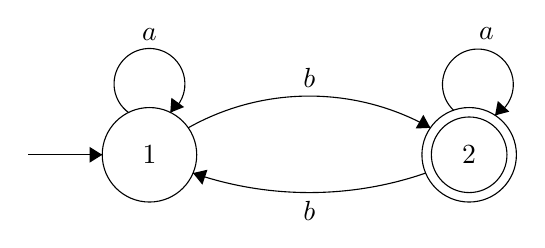
\begin{tikzpicture}[scale=0.2]
\tikzstyle{every node}+=[inner sep=0pt]
\draw [black] (8.5,-9.7) circle (3);
\draw (8.5,-9.7) node {$1$};
\draw [black] (28.8,-9.7) circle (3);
\draw (28.8,-9.7) node {$2$};
\draw [black] (28.8,-9.7) circle (2.4);
\draw [black] (0.8,-9.7) -- (5.5,-9.7);
\fill [black] (5.5,-9.7) -- (4.7,-9.2) -- (4.7,-10.2);
\draw [black] (7.177,-7.02) arc (234:-54:2.25);
\draw (8.5,-2.45) node [above] {$a$};
\fill [black] (9.82,-7.02) -- (10.7,-6.67) -- (9.89,-6.08);
\draw [black] (10.958,-7.988) arc (119.38377:60.61623:15.677);
\fill [black] (26.34,-7.99) -- (25.89,-7.16) -- (25.4,-8.03);
\draw (18.65,-5.47) node [above] {$b$};
\draw [black] (26.037,-10.862) arc (-70.97721:-109.02279:22.663);
\fill [black] (11.26,-10.86) -- (11.86,-11.6) -- (12.18,-10.65);
\draw (18.65,-12.6) node [below] {$b$};
\draw [black] (27.818,-6.878) arc (226.92001:-61.07999:2.25);
\draw (29.89,-2.42) node [above] {$a$};
\fill [black] (30.44,-7.2) -- (31.35,-6.96) -- (30.62,-6.28);
\end{tikzpicture}
\end{center}
\pagebreak
1. Turn it into GNFA
\begin{center}
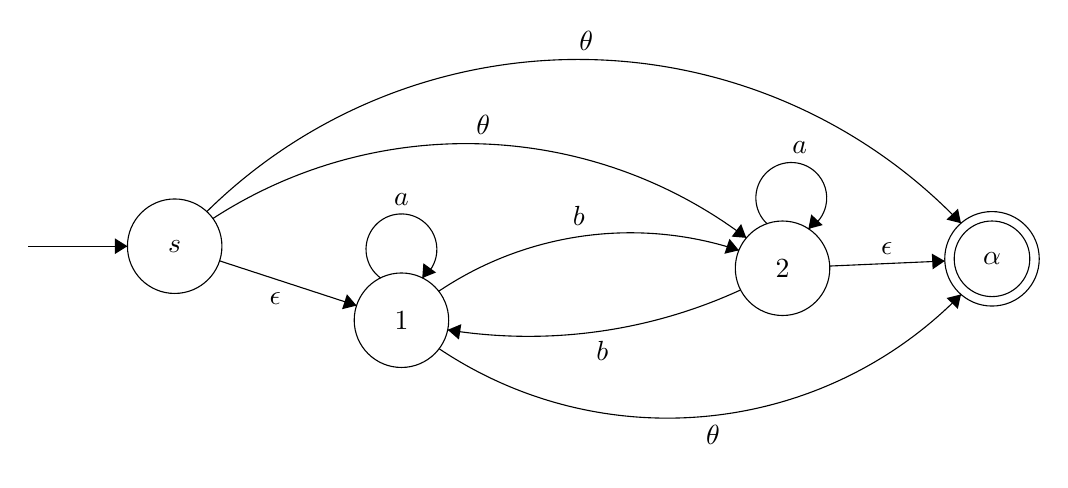
\begin{tikzpicture}[scale=0.2]
\tikzstyle{every node}+=[inner sep=0pt]
\draw [black] (28.7,-19.7) circle (3);
\draw (28.7,-19.7) node {$1$};
\draw [black] (52.9,-16.4) circle (3);
\draw (52.9,-16.4) node {$2$};
\draw [black] (14.3,-15) circle (3);
\draw (14.3,-15) node {$s$};
\draw [black] (66.2,-15.8) circle (3);
\draw (66.2,-15.8) node {$\alpha$};
\draw [black] (66.2,-15.8) circle (2.4);
\draw [black] (27.377,-17.02) arc (234:-54:2.25);
\draw (28.7,-12.45) node [above] {$a$};
\fill [black] (30.02,-17.02) -- (30.9,-16.67) -- (30.09,-16.08);
\draw [black] (31.067,-17.86) arc (123.92448:71.60585:21.817);
\fill [black] (50.13,-15.26) -- (49.53,-14.53) -- (49.21,-15.48);
\draw (39.97,-13.75) node [above] {$b$};
\draw [black] (50.236,-17.777) arc (-65.32404:-99.14563:32.269);
\fill [black] (31.64,-20.31) -- (32.35,-20.93) -- (32.5,-19.95);
\draw (41.45,-21.02) node [below] {$b$};
\draw [black] (51.918,-13.578) arc (226.92001:-61.07999:2.25);
\draw (53.99,-9.12) node [above] {$a$};
\fill [black] (54.54,-13.9) -- (55.45,-13.66) -- (54.72,-12.98);
\draw [black] (17.15,-15.93) -- (25.85,-18.77);
\fill [black] (25.85,-18.77) -- (25.24,-18.05) -- (24.93,-19);
\draw (20.69,-17.89) node [below] {$\epsilon$};
\draw [black] (5,-15) -- (11.3,-15);
\fill [black] (11.3,-15) -- (10.5,-14.5) -- (10.5,-15.5);
\draw [black] (55.9,-16.26) -- (63.2,-15.94);
\fill [black] (63.2,-15.94) -- (62.38,-15.47) -- (62.43,-16.47);
\draw (59.51,-15.56) node [above] {$\epsilon$};
\draw [black] (64.233,-18.063) arc (-44.30007:-123.82509:26.048);
\fill [black] (64.23,-18.06) -- (63.32,-18.29) -- (64.03,-18.98);
\draw (48.48,-26.36) node [below] {$\theta$};
\draw [black] (16.341,-12.802) arc (134.56517:43.66863:33.604);
\fill [black] (64.23,-13.54) -- (64.04,-12.62) -- (63.31,-13.31);
\draw (40.44,-2.63) node [above] {$\theta$};
\draw [black] (16.729,-13.241) arc (122.99256:52.85309:29.499);
\fill [black] (50.6,-14.47) -- (50.27,-13.59) -- (49.67,-14.39);
\draw (33.89,-7.97) node [above] {$\theta$};
\end{tikzpicture}
\end{center}

2. Rip state 1 out, and repair the connections.
\begin{center}
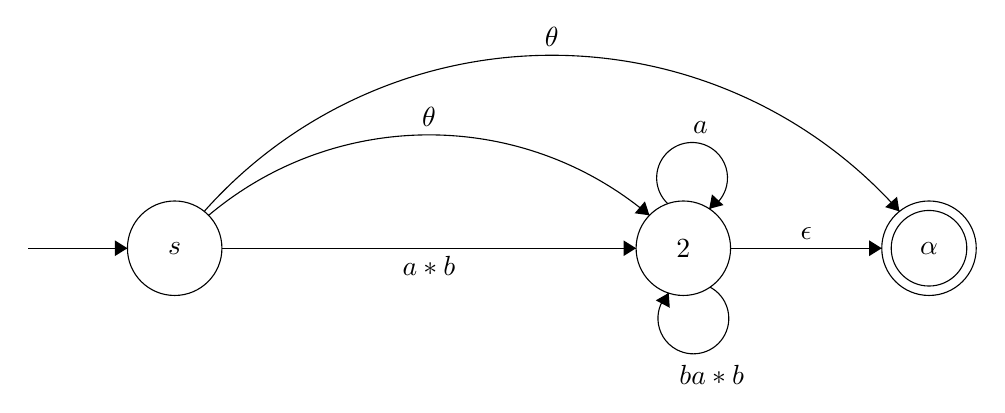
\begin{tikzpicture}[scale=0.2]
\tikzstyle{every node}+=[inner sep=0pt]
\draw [black] (46.6,-15) circle (3);
\draw (46.6,-15) node {$2$};
\draw [black] (14.3,-15) circle (3);
\draw (14.3,-15) node {$s$};
\draw [black] (62.2,-15) circle (3);
\draw (62.2,-15) node {$\alpha$};
\draw [black] (62.2,-15) circle (2.4);
\draw [black] (45.618,-12.178) arc (226.92001:-61.07999:2.25);
\draw (47.69,-7.72) node [above] {$a$};
\fill [black] (48.24,-12.5) -- (49.15,-12.26) -- (48.42,-11.58);
\draw [black] (5,-15) -- (11.3,-15);
\fill [black] (11.3,-15) -- (10.5,-14.5) -- (10.5,-15.5);
\draw [black] (49.6,-15) -- (59.2,-15);
\fill [black] (59.2,-15) -- (58.4,-14.5) -- (58.4,-15.5);
\draw (54.4,-14.5) node [above] {$\epsilon$};
\draw [black] (16.176,-12.66) arc (138.37374:41.62626:29.531);
\fill [black] (60.32,-12.66) -- (60.17,-11.73) -- (59.42,-12.39);
\draw (38.25,-2.25) node [above] {$\theta$};
\draw [black] (16.453,-12.914) arc (130.13427:49.86573:21.715);
\fill [black] (44.45,-12.91) -- (44.16,-12.02) -- (43.51,-12.78);
\draw (30.45,-7.3) node [above] {$\theta$};
\draw [black] (17.3,-15) -- (43.6,-15);
\fill [black] (43.6,-15) -- (42.8,-14.5) -- (42.8,-15.5);
\draw (30.45,-15.5) node [below] {$a*b$};
\draw [black] (48.288,-17.466) arc (62.1301:-225.8699:2.25);
\draw (48.4,-22.41) node [below] {$ba*b$};
\fill [black] (45.67,-17.84) -- (44.85,-18.31) -- (45.74,-18.78);
\end{tikzpicture}
\end{center}

\begin{center}
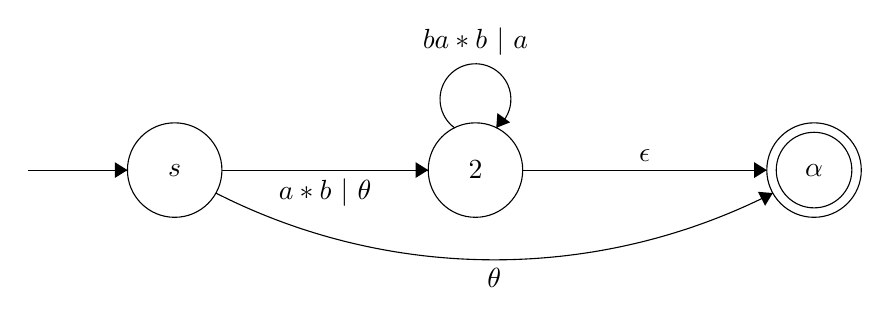
\begin{tikzpicture}[scale=0.2]
\tikzstyle{every node}+=[inner sep=0pt]
\draw [black] (31.6,-9.7) circle (3);
\draw (31.6,-9.7) node {$2$};
\draw [black] (12.5,-9.7) circle (3);
\draw (12.5,-9.7) node {$s$};
\draw [black] (53.1,-9.7) circle (3);
\draw (53.1,-9.7) node {$\alpha$};
\draw [black] (53.1,-9.7) circle (2.4);
\draw [black] (3.2,-9.7) -- (9.5,-9.7);
\fill [black] (9.5,-9.7) -- (8.7,-9.2) -- (8.7,-10.2);
\draw [black] (34.6,-9.7) -- (50.1,-9.7);
\fill [black] (50.1,-9.7) -- (49.3,-9.2) -- (49.3,-10.2);
\draw (42.35,-9.2) node [above] {$\epsilon$};
\draw [black] (50.481,-11.162) arc (-63.03923:-116.96077:38.998);
\fill [black] (50.48,-11.16) -- (49.54,-11.08) -- (49.99,-11.97);
\draw (32.8,-15.9) node [below] {$\theta$};
\draw [black] (15.5,-9.7) -- (28.6,-9.7);
\fill [black] (28.6,-9.7) -- (27.8,-9.2) -- (27.8,-10.2);
\draw (22.05,-10.2) node [below] {$a*b\mbox{ }|\mbox{ }\theta$};
\draw [black] (30.277,-7.02) arc (234:-54:2.25);
\draw (31.6,-2.45) node [above] {$ba*b\mbox{ }|\mbox{ }a$};
\fill [black] (32.92,-7.02) -- (33.8,-6.67) -- (32.99,-6.08);
\end{tikzpicture}
\end{center}

3. Rip state 2 out, and repair the connections.
\begin{center}
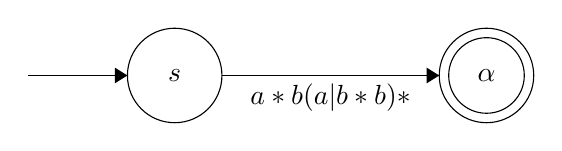
\begin{tikzpicture}[scale=0.2]
\tikzstyle{every node}+=[inner sep=0pt]
\draw [black] (12.5,-9.7) circle (3);
\draw (12.5,-9.7) node {$s$};
\draw [black] (32.3,-9.7) circle (3);
\draw (32.3,-9.7) node {$\alpha$};
\draw [black] (32.3,-9.7) circle (2.4);
\draw [black] (3.2,-9.7) -- (9.5,-9.7);
\fill [black] (9.5,-9.7) -- (8.7,-9.2) -- (8.7,-10.2);
\draw [black] (15.5,-9.7) -- (29.3,-9.7);
\fill [black] (29.3,-9.7) -- (28.5,-9.2) -- (28.5,-10.2);
\draw (22.4,-10.2) node [below] {$a*b(a|b*b)*$};
\end{tikzpicture}
\end{center}

\answ{$a^*b(a|b^bb)^*$}

\pagebreak

\problem{1.21 b}

\begin{center}
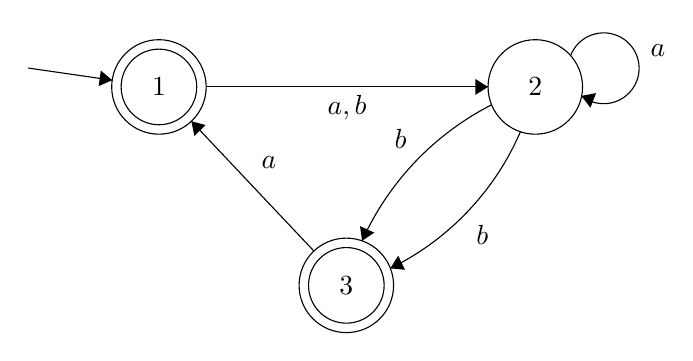
\begin{tikzpicture}[scale=0.2]
\tikzstyle{every node}+=[inner sep=0pt]
\draw [black] (9.7,-4.7) circle (3);
\draw (9.7,-4.7) node {$1$};
\draw [black] (9.7,-4.7) circle (2.4);
\draw [black] (33.6,-4.7) circle (3);
\draw (33.6,-4.7) node {$2$};
\draw [black] (21.6,-17.3) circle (3);
\draw (21.6,-17.3) node {$3$};
\draw [black] (21.6,-17.3) circle (2.4);
\draw [black] (1.4,-3.5) -- (6.73,-4.27);
\fill [black] (6.73,-4.27) -- (6.01,-3.66) -- (5.87,-4.65);
\draw [black] (12.7,-4.7) -- (30.6,-4.7);
\fill [black] (30.6,-4.7) -- (29.8,-4.2) -- (29.8,-5.2);
\draw (21.65,-5.2) node [below] {$a,b$};
\draw [black] (35.837,-2.719) arc (159.25512:-128.74488:2.25);
\draw (40.88,-2.4) node [right] {$a$};
\fill [black] (36.53,-5.27) -- (37.1,-6.02) -- (37.46,-5.09);
\draw [black] (32.655,-7.543) arc (-23.34366:-63.86198:17.297);
\fill [black] (24.39,-16.22) -- (25.33,-16.31) -- (24.89,-15.42);
\draw (29.83,-14.09) node [right] {$b$};
\draw [black] (22.598,-14.475) arc (155.76965:117.02471:17.985);
\fill [black] (22.6,-14.47) -- (23.38,-13.95) -- (22.47,-13.54);
\draw (25.45,-7.98) node [left] {$b$};
\draw [black] (19.54,-15.12) -- (11.76,-6.88);
\fill [black] (11.76,-6.88) -- (11.95,-7.81) -- (12.67,-7.12);
\draw (16.18,-9.53) node [right] {$a$};
\end{tikzpicture}
\end{center}


1. Convert DFA to GNFA.
\begin{center}
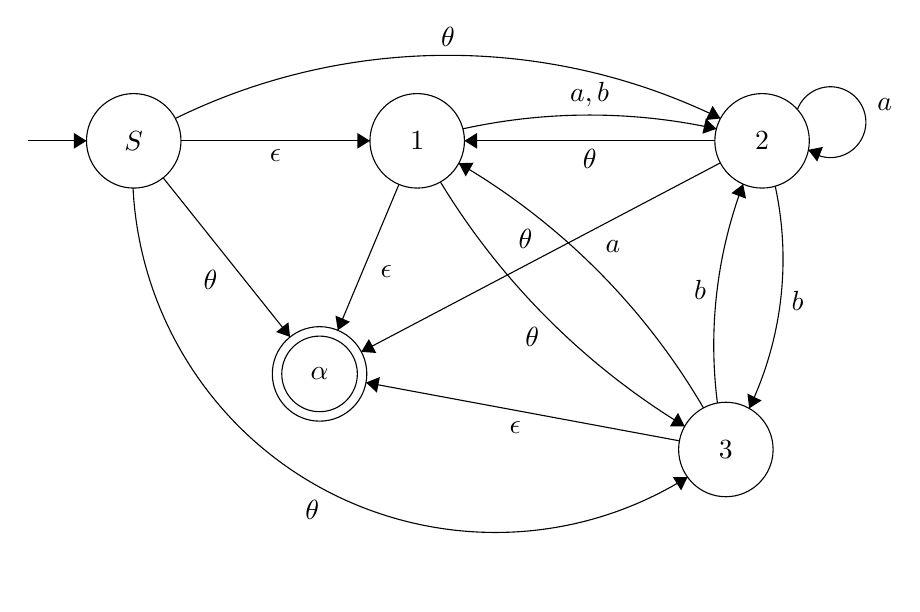
\begin{tikzpicture}[scale=0.2]
\tikzstyle{every node}+=[inner sep=0pt]
\draw [black] (27.4,-10.5) circle (3);
\draw (27.4,-10.5) node {$1$};
\draw [black] (49.3,-10.5) circle (3);
\draw (49.3,-10.5) node {$2$};
\draw [black] (47,-30.1) circle (3);
\draw (47,-30.1) node {$3$};
\draw [black] (21.2,-25.3) circle (3);
\draw (21.2,-25.3) node {$\alpha$};
\draw [black] (21.2,-25.3) circle (2.4);
\draw [black] (9.4,-10.5) circle (3);
\draw (9.4,-10.5) node {$S$};
\draw [black] (30.301,-9.738) arc (102.42151:77.57849:37.42);
\fill [black] (46.4,-9.74) -- (45.73,-9.08) -- (45.51,-10.05);
\draw (38.35,-8.36) node [above] {$a,b$};
\draw [black] (51.537,-8.519) arc (159.25512:-128.74488:2.25);
\draw (56.58,-8.2) node [right] {$a$};
\fill [black] (52.23,-11.07) -- (52.8,-11.82) -- (53.16,-10.89);
\draw [black] (50.134,-13.379) arc (12.22469:-25.61044:21.914);
\fill [black] (48.48,-27.49) -- (49.27,-26.99) -- (48.37,-26.55);
\draw (51.14,-20.69) node [right] {$b$};
\draw [black] (30.041,-11.923) arc (59.69881:30.30119:43.297);
\fill [black] (30.04,-11.92) -- (30.48,-12.76) -- (30.98,-11.89);
\draw (39.33,-17.21) node [right] {$a$};
\draw [black] (44.05,-29.55) -- (24.15,-25.85);
\fill [black] (24.15,-25.85) -- (24.84,-26.49) -- (25.03,-25.5);
\draw (33.63,-28.28) node [below] {$\epsilon$};
\draw [black] (26.24,-13.27) -- (22.36,-22.53);
\fill [black] (22.36,-22.53) -- (23.13,-21.99) -- (22.21,-21.6);
\draw (25.04,-18.83) node [right] {$\epsilon$};
\draw [black] (12.4,-10.5) -- (24.4,-10.5);
\fill [black] (24.4,-10.5) -- (23.6,-10) -- (23.6,-11);
\draw (18.4,-11) node [below] {$\epsilon$};
\draw [black] (2.7,-10.5) -- (6.4,-10.5);
\fill [black] (6.4,-10.5) -- (5.6,-10) -- (5.6,-11);
\draw [black] (12.041,-9.079) arc (116.09472:63.90528:39.351);
\fill [black] (46.66,-9.08) -- (46.16,-8.28) -- (45.72,-9.18);
\draw (29.35,-4.57) node [above] {$\theta$};
\draw [black] (44.388,-28.626) arc (-121.2923:-148.7077:46.292);
\fill [black] (44.39,-28.63) -- (43.96,-27.78) -- (43.44,-28.64);
\draw (34.7,-22.28) node [below] {$\theta$};
\draw [black] (46.465,-27.149) arc (-172.70075:-200.685:28.947);
\fill [black] (48.1,-13.25) -- (47.35,-13.82) -- (48.28,-14.17);
\draw (45.77,-19.98) node [left] {$b$};
\draw [black] (44.568,-31.854) arc (-57.93537:-177.12858:23.021);
\fill [black] (44.57,-31.85) -- (43.63,-31.85) -- (44.16,-32.7);
\draw (20.73,-33.26) node [below] {$\theta$};
\draw [black] (11.27,-12.85) -- (19.33,-22.95);
\fill [black] (19.33,-22.95) -- (19.22,-22.02) -- (18.44,-22.64);
\draw (14.74,-19.32) node [left] {$\theta$};
\draw [black] (46.3,-10.5) -- (30.4,-10.5);
\fill [black] (30.4,-10.5) -- (31.2,-11) -- (31.2,-10);
\draw (38.35,-11) node [below] {$\theta$};
\draw [black] (46.65,-11.9) -- (23.85,-23.9);
\fill [black] (23.85,-23.9) -- (24.8,-23.97) -- (24.33,-23.09);
\draw (34.28,-17.4) node [above] {$\theta$};
\end{tikzpicture}
\end{center}

2. Rip state 1 out, and repair connections.

\begin{center}
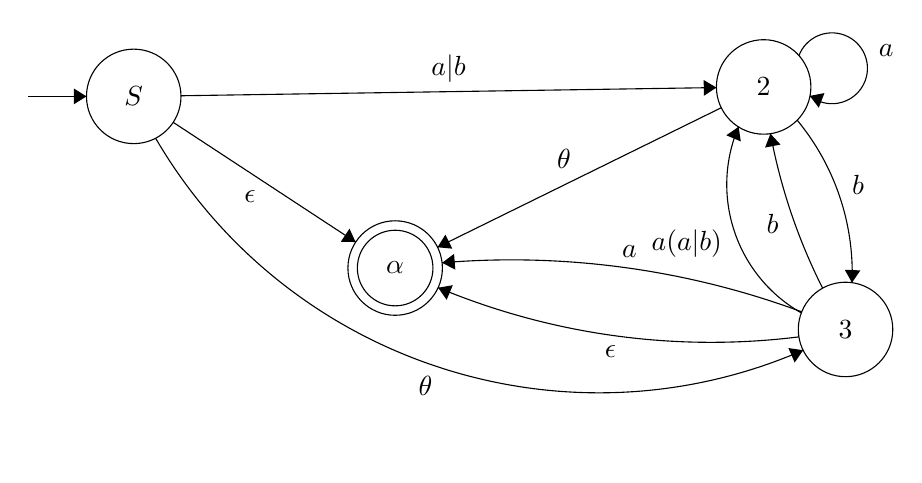
\begin{tikzpicture}[scale=0.2]
\tikzstyle{every node}+=[inner sep=0pt]
\draw [black] (48.6,-4.6) circle (3);
\draw (48.6,-4.6) node {$2$};
\draw [black] (53.8,-20) circle (3);
\draw (53.8,-20) node {$3$};
\draw [black] (25.2,-16.1) circle (3);
\draw (25.2,-16.1) node {$\alpha$};
\draw [black] (25.2,-16.1) circle (2.4);
\draw [black] (8.6,-5.2) circle (3);
\draw (8.6,-5.2) node {$S$};
\draw [black] (50.837,-2.619) arc (159.25512:-128.74488:2.25);
\draw (55.88,-2.3) node [right] {$a$};
\fill [black] (51.53,-5.17) -- (52.1,-5.92) -- (52.46,-4.99);
\draw [black] (50.727,-6.709) arc (39.59956:-2.28379:15.244);
\fill [black] (54.21,-17.03) -- (54.74,-16.25) -- (53.75,-16.21);
\draw (54.19,-10.83) node [right] {$b$};
\draw [black] (28.181,-15.765) arc (94.78721:69.68246:53.025);
\fill [black] (28.18,-15.77) -- (29.02,-16.2) -- (28.94,-15.2);
\draw (40.07,-15.48) node [above] {$a$};
\draw [black] (1.9,-5.2) -- (5.6,-5.2);
\fill [black] (5.6,-5.2) -- (4.8,-4.7) -- (4.8,-5.7);
\draw [black] (11.6,-5.16) -- (45.6,-4.64);
\fill [black] (45.6,-4.64) -- (44.79,-4.16) -- (44.81,-5.16);
\draw (28.59,-4.38) node [above] {$a|b$};
\draw [black] (52.343,-17.379) arc (-153.26269:-169.42153:36.837);
\fill [black] (49.03,-7.57) -- (48.69,-8.45) -- (49.67,-8.26);
\draw (49.58,-13.31) node [left] {$b$};
\draw [black] (51.107,-21.321) arc (-66.51217:-149.7482:32.572);
\fill [black] (51.11,-21.32) -- (50.17,-21.18) -- (50.57,-22.1);
\draw (27.13,-22.94) node [below] {$\theta$};
\draw [black] (45.91,-5.92) -- (27.89,-14.78);
\fill [black] (27.89,-14.78) -- (28.83,-14.87) -- (28.39,-13.98);
\draw (35.93,-9.84) node [above] {$\theta$};
\draw [black] (11.11,-6.85) -- (22.69,-14.45);
\fill [black] (22.69,-14.45) -- (22.3,-13.6) -- (21.75,-14.43);
\draw (15.98,-11.15) node [below] {$\epsilon$};
\draw [black] (50.838,-20.471) arc (-82.88423:-112.6461:45.017);
\fill [black] (27.93,-17.35) -- (28.47,-18.12) -- (28.86,-17.19);
\draw (38.88,-20.99) node [below] {$\epsilon$};
\draw [black] (51.001,-18.955) arc (-119.62903:-203.05519:9.381);
\fill [black] (47.01,-7.13) -- (46.23,-7.67) -- (47.15,-8.06);
\draw (45.99,-14.52) node [left] {$a(a|b)$};
\end{tikzpicture}
\end{center}

\pagebreak

3. Unite multiple connections.
\begin{center}
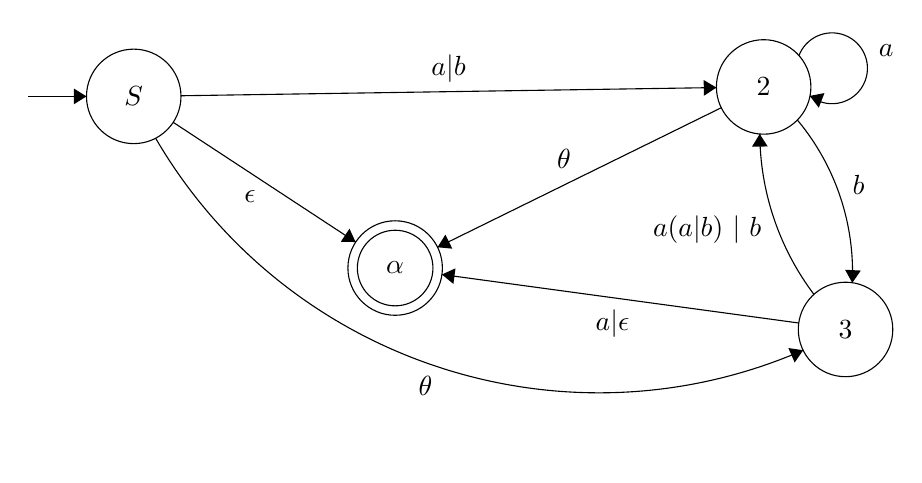
\begin{tikzpicture}[scale=0.2]
\tikzstyle{every node}+=[inner sep=0pt]
\draw [black] (48.6,-4.6) circle (3);
\draw (48.6,-4.6) node {$2$};
\draw [black] (53.8,-20) circle (3);
\draw (53.8,-20) node {$3$};
\draw [black] (25.2,-16.1) circle (3);
\draw (25.2,-16.1) node {$\alpha$};
\draw [black] (25.2,-16.1) circle (2.4);
\draw [black] (8.6,-5.2) circle (3);
\draw (8.6,-5.2) node {$S$};
\draw [black] (50.837,-2.619) arc (159.25512:-128.74488:2.25);
\draw (55.88,-2.3) node [right] {$a$};
\fill [black] (51.53,-5.17) -- (52.1,-5.92) -- (52.46,-4.99);
\draw [black] (50.739,-6.697) arc (39.87058:-2.5548:15.08);
\fill [black] (54.23,-17.04) -- (54.77,-16.26) -- (53.77,-16.21);
\draw (54.22,-10.82) node [right] {$b$};
\draw [black] (1.9,-5.2) -- (5.6,-5.2);
\fill [black] (5.6,-5.2) -- (4.8,-4.7) -- (4.8,-5.7);
\draw [black] (11.6,-5.16) -- (45.6,-4.64);
\fill [black] (45.6,-4.64) -- (44.79,-4.16) -- (44.81,-5.16);
\draw (28.59,-4.38) node [above] {$a|b$};
\draw [black] (51.107,-21.321) arc (-66.51217:-149.7482:32.572);
\fill [black] (51.11,-21.32) -- (50.17,-21.18) -- (50.57,-22.1);
\draw (27.13,-22.94) node [below] {$\theta$};
\draw [black] (45.91,-5.92) -- (27.89,-14.78);
\fill [black] (27.89,-14.78) -- (28.83,-14.87) -- (28.39,-13.98);
\draw (35.93,-9.84) node [above] {$\theta$};
\draw [black] (11.11,-6.85) -- (22.69,-14.45);
\fill [black] (22.69,-14.45) -- (22.3,-13.6) -- (21.75,-14.43);
\draw (15.98,-11.15) node [below] {$\epsilon$};
\draw [black] (50.83,-19.59) -- (28.17,-16.51);
\fill [black] (28.17,-16.51) -- (28.9,-17.11) -- (29.03,-16.12);
\draw (39,-18.69) node [below] {$a|\epsilon$};
\draw [black] (51.794,-17.774) arc (-143.00883:-179.67539:17.093);
\fill [black] (48.35,-7.59) -- (47.86,-8.39) -- (48.86,-8.38);
\draw (48.49,-13.67) node [left] {$a(a|b)\mbox{ }|\mbox{ }b$};
\end{tikzpicture}
\end{center}

4. Rip out state 2, and repair broken edges.
\begin{center}
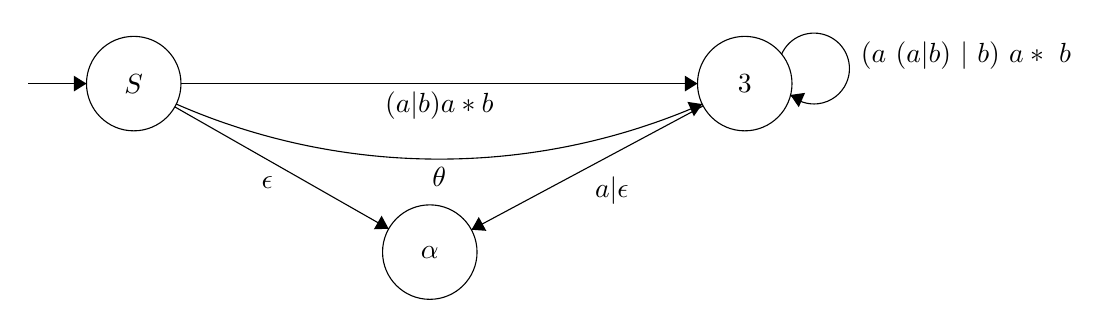
\begin{tikzpicture}[scale=0.2]
\tikzstyle{every node}+=[inner sep=0pt]
\draw [black] (48.4,-5.5) circle (3);
\draw (48.4,-5.5) node {$3$};
\draw [black] (28.4,-16.2) circle (3);
\draw (28.4,-16.2) node {$\alpha$};
\draw [black] (9.6,-5.5) circle (3);
\draw (9.6,-5.5) node {$S$};
\draw [black] (2.9,-5.5) -- (6.6,-5.5);
\fill [black] (6.6,-5.5) -- (5.8,-5) -- (5.8,-6);
\draw [black] (45.697,-6.801) arc (-66.35803:-113.64197:41.638);
\fill [black] (45.7,-6.8) -- (44.76,-6.66) -- (45.17,-7.58);
\draw (29,-10.8) node [below] {$\theta$};
\draw [black] (12.21,-6.98) -- (25.79,-14.72);
\fill [black] (25.79,-14.72) -- (25.34,-13.89) -- (24.85,-14.75);
\draw (18.08,-11.35) node [below] {$\epsilon$};
\draw [black] (45.75,-6.92) -- (31.05,-14.78);
\fill [black] (31.05,-14.78) -- (31.99,-14.85) -- (31.51,-13.97);
\draw (39.96,-11.35) node [below] {$a|\epsilon$};
\draw [black] (12.6,-5.5) -- (45.4,-5.5);
\fill [black] (45.4,-5.5) -- (44.6,-5) -- (44.6,-6);
\draw (29,-6) node [below] {$(a|b)a*b$};
\draw [black] (50.738,-3.638) arc (156.26477:-131.73523:2.25);
\draw (55.74,-3.7) node [right] {$(a\mbox{ }(a|b)\mbox{ }|\mbox{ }b)\mbox{ }a*\mbox{ }b$};
\fill [black] (51.3,-6.22) -- (51.83,-7) -- (52.23,-6.09);
\end{tikzpicture}
\end{center}

5. Rip out state 3 and repair broken edges.
\begin{center}
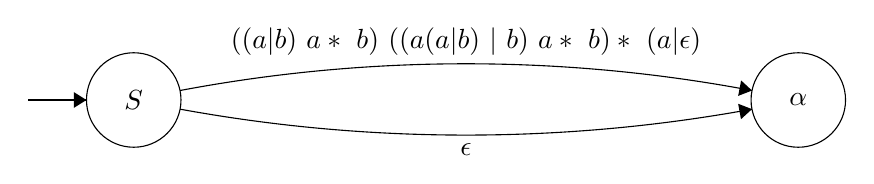
\begin{tikzpicture}[scale=0.2]
\tikzstyle{every node}+=[inner sep=0pt]
\draw [black] (51.4,-6.6) circle (3);
\draw (51.4,-6.6) node {$\alpha$};
\draw [black] (9.2,-6.6) circle (3);
\draw (9.2,-6.6) node {$S$};
\draw [black] (2.5,-6.6) -- (6.2,-6.6);
\fill [black] (6.2,-6.6) -- (5.4,-6.1) -- (5.4,-7.1);
\draw [black] (48.457,-7.183) arc (-79.64369:-100.35631:101.004);
\fill [black] (48.46,-7.18) -- (47.58,-6.84) -- (47.76,-7.82);
\draw (30.3,-9.33) node [below] {$\epsilon$};
\draw [black] (12.139,-5.998) arc (100.69413:79.30587:97.869);
\fill [black] (48.46,-6) -- (47.77,-5.36) -- (47.58,-6.34);
\draw (30.3,-3.8) node [above] {$((a|b)\mbox{ }a*\mbox{ }b)\mbox{ }((a(a|b)\mbox{ }|\mbox{ }b)\mbox{ }a*\mbox{ }b)*\mbox{ }(a|\epsilon)$};
\end{tikzpicture}
\end{center}

6. Unite the edges.
\begin{center}
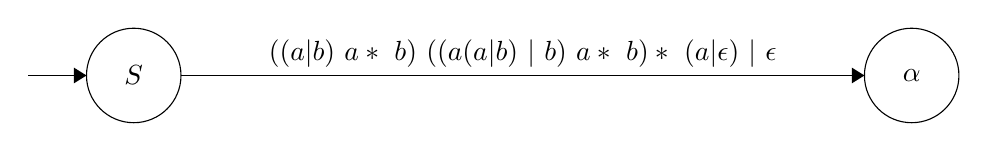
\begin{tikzpicture}[scale=0.2]
\tikzstyle{every node}+=[inner sep=0pt]
\draw [black] (58.2,-4.4) circle (3);
\draw (58.2,-4.4) node {$\alpha$};
\draw [black] (8.8,-4.4) circle (3);
\draw (8.8,-4.4) node {$S$};
\draw [black] (2.1,-4.4) -- (5.8,-4.4);
\fill [black] (5.8,-4.4) -- (5,-3.9) -- (5,-4.9);
\draw [black] (11.8,-4.4) -- (55.2,-4.4);
\fill [black] (55.2,-4.4) -- (54.4,-3.9) -- (54.4,-4.9);
\draw (33.5,-3.9) node [above] {$((a|b)\mbox{ }a*\mbox{ }b)\mbox{ }((a(a|b)\mbox{ }|\mbox{ }b)\mbox{ }a*\mbox{ }b)*\mbox{ }(a|\epsilon)\mbox{ }|\mbox{ }\epsilon$};
\end{tikzpicture}
\end{center}

\vspace{1cm}
\answ{$((a | b) a^* b) ((a (a|b) | b) a^* b)^* (a | \epsilon ) | \epsilon$}

\pagebreak

\problem{1.28}
Convert the following regular expression to NFA using the procedure given in Theorem 1.54.
In all parts, $\sum = \{a,b\}$. \\ \\
\problem{1.28 b}

$a^+ | (ab)^+$ \\

1. NFA that recognizes symbol $a$.
\begin{center}
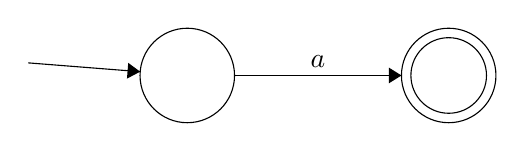
\begin{tikzpicture}[scale=0.2]
\tikzstyle{every node}+=[inner sep=0pt]
\draw [black] (13.3,-6) circle (3);
\draw [black] (29.9,-6) circle (3);
\draw [black] (29.9,-6) circle (2.4);
\draw [black] (3.2,-5.2) -- (10.31,-5.76);
\fill [black] (10.31,-5.76) -- (9.55,-5.2) -- (9.47,-6.2);
\draw [black] (16.3,-6) -- (26.9,-6);
\fill [black] (26.9,-6) -- (26.1,-5.5) -- (26.1,-6.5);
\draw (21.6,-5.5) node [above] {$a$};
\end{tikzpicture}
\end{center}

2. NFA that recognizes symbol $b$.
\begin{center}
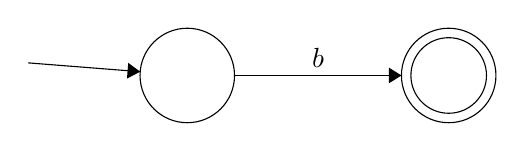
\begin{tikzpicture}[scale=0.2]
\tikzstyle{every node}+=[inner sep=0pt]
\draw [black] (13.3,-6) circle (3);
\draw [black] (29.9,-6) circle (3);
\draw [black] (29.9,-6) circle (2.4);
\draw [black] (3.2,-5.2) -- (10.31,-5.76);
\fill [black] (10.31,-5.76) -- (9.55,-5.2) -- (9.47,-6.2);
\draw [black] (16.3,-6) -- (26.9,-6);
\fill [black] (26.9,-6) -- (26.1,-5.5) -- (26.1,-6.5);
\draw (21.6,-5.5) node [above] {$b$};
\end{tikzpicture}
\end{center}

3. NFA that recognizes concatenation of 1 and 2, i.e string $ab$.
\begin{center}
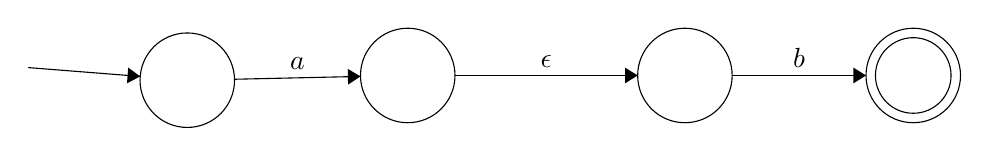
\begin{tikzpicture}[scale=0.2]
\tikzstyle{every node}+=[inner sep=0pt]
\draw [black] (13.3,-6) circle (3);
\draw [black] (27.3,-5.7) circle (3);
\draw [black] (44.9,-5.7) circle (3);
\draw [black] (59.4,-5.7) circle (3);
\draw [black] (59.4,-5.7) circle (2.4);
\draw [black] (3.2,-5.2) -- (10.31,-5.76);
\fill [black] (10.31,-5.76) -- (9.55,-5.2) -- (9.47,-6.2);
\draw [black] (16.3,-5.94) -- (24.3,-5.76);
\fill [black] (24.3,-5.76) -- (23.49,-5.28) -- (23.51,-6.28);
\draw (20.29,-5.33) node [above] {$a$};
\draw [black] (30.3,-5.7) -- (41.9,-5.7);
\fill [black] (41.9,-5.7) -- (41.1,-5.2) -- (41.1,-6.2);
\draw (36.1,-5.2) node [above] {$\epsilon$};
\draw [black] (47.9,-5.7) -- (56.4,-5.7);
\fill [black] (56.4,-5.7) -- (55.6,-5.2) -- (55.6,-6.2);
\draw (52.15,-5.2) node [above] {$b$};
\end{tikzpicture}
\end{center}

4. NFA that recognizes regular expression $(ab)^+$.
\begin{center}
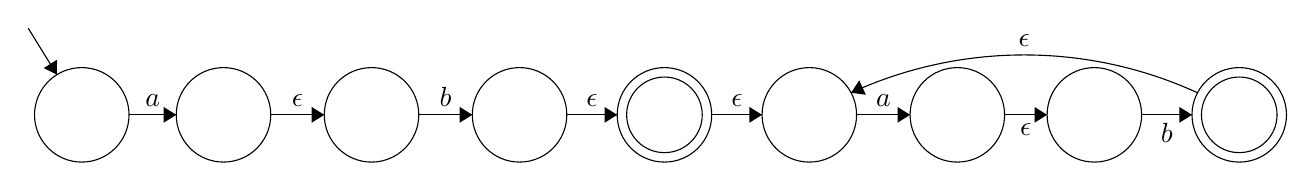
\begin{tikzpicture}[scale=0.2]
\tikzstyle{every node}+=[inner sep=0pt]
\draw [black] (3.4,-6.3) circle (3);
\draw [black] (12.4,-6.3) circle (3);
\draw [black] (21.8,-6.3) circle (3);
\draw [black] (31.2,-6.3) circle (3);
\draw [black] (40.4,-6.3) circle (3);
\draw [black] (40.4,-6.3) circle (2.4);
\draw [black] (67.7,-6.3) circle (3);
\draw [black] (76.9,-6.3) circle (3);
\draw [black] (76.9,-6.3) circle (2.4);
\draw [black] (49.6,-6.3) circle (3);
\draw [black] (59,-6.3) circle (3);
\draw [black] (0,-0.8) -- (1.82,-3.75);
\fill [black] (1.82,-3.75) -- (1.83,-2.8) -- (0.98,-3.33);
\draw [black] (6.4,-6.3) -- (9.4,-6.3);
\fill [black] (9.4,-6.3) -- (8.6,-5.8) -- (8.6,-6.8);
\draw (7.9,-5.8) node [above] {$a$};
\draw [black] (15.4,-6.3) -- (18.8,-6.3);
\fill [black] (18.8,-6.3) -- (18,-5.8) -- (18,-6.8);
\draw (17.1,-5.8) node [above] {$\epsilon$};
\draw [black] (24.8,-6.3) -- (28.2,-6.3);
\fill [black] (28.2,-6.3) -- (27.4,-5.8) -- (27.4,-6.8);
\draw (26.5,-5.8) node [above] {$b$};
\draw [black] (34.2,-6.3) -- (37.4,-6.3);
\fill [black] (37.4,-6.3) -- (36.6,-5.8) -- (36.6,-6.8);
\draw (35.8,-5.8) node [above] {$\epsilon$};
\draw [black] (70.7,-6.3) -- (73.9,-6.3);
\fill [black] (73.9,-6.3) -- (73.1,-5.8) -- (73.1,-6.8);
\draw (72.3,-6.8) node [below] {$b$};
\draw [black] (43.4,-6.3) -- (46.6,-6.3);
\fill [black] (46.6,-6.3) -- (45.8,-5.8) -- (45.8,-6.8);
\draw (45,-5.8) node [above] {$\epsilon$};
\draw [black] (52.6,-6.3) -- (56,-6.3);
\fill [black] (56,-6.3) -- (55.2,-5.8) -- (55.2,-6.8);
\draw (54.3,-5.8) node [above] {$a$};
\draw [black] (62,-6.3) -- (64.7,-6.3);
\fill [black] (64.7,-6.3) -- (63.9,-5.8) -- (63.9,-6.8);
\draw (63.35,-6.8) node [below] {$\epsilon$};
\draw [black] (52.25,-4.897) arc (114.63693:65.36307:26.387);
\fill [black] (52.25,-4.9) -- (53.19,-5.02) -- (52.77,-4.11);
\draw (63.25,-2) node [above] {$\epsilon$};
\end{tikzpicture}
\end{center}


5. NFA that recognizes regular expression $(a)^+$.
\begin{center}
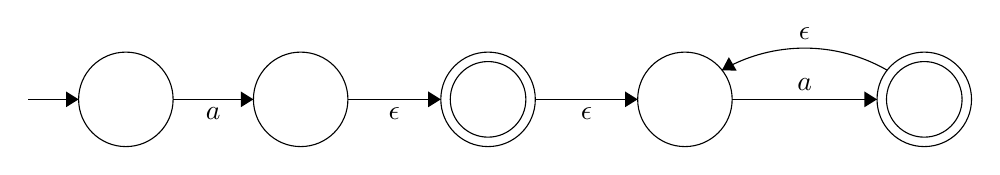
\begin{tikzpicture}[scale=0.2]
\tikzstyle{every node}+=[inner sep=0pt]
\draw [black] (7.7,-6.1) circle (3);
\draw [black] (18.8,-6.1) circle (3);
\draw [black] (30.7,-6.1) circle (3);
\draw [black] (30.7,-6.1) circle (2.4);
\draw [black] (43.2,-6.1) circle (3);
\draw [black] (58.4,-6.1) circle (3);
\draw [black] (58.4,-6.1) circle (2.4);
\draw [black] (10.7,-6.1) -- (15.8,-6.1);
\fill [black] (15.8,-6.1) -- (15,-5.6) -- (15,-6.6);
\draw (13.25,-6.6) node [below] {$a$};
\draw [black] (21.8,-6.1) -- (27.7,-6.1);
\fill [black] (27.7,-6.1) -- (26.9,-5.6) -- (26.9,-6.6);
\draw (24.75,-6.6) node [below] {$\epsilon$};
\draw [black] (33.7,-6.1) -- (40.2,-6.1);
\fill [black] (40.2,-6.1) -- (39.4,-5.6) -- (39.4,-6.6);
\draw (36.95,-6.6) node [below] {$\epsilon$};
\draw [black] (46.2,-6.1) -- (55.4,-6.1);
\fill [black] (55.4,-6.1) -- (54.6,-5.6) -- (54.6,-6.6);
\draw (50.8,-5.6) node [above] {$a$};
\draw [black] (45.55,-4.252) arc (120.00385:59.99615:10.499);
\fill [black] (45.55,-4.25) -- (46.49,-4.28) -- (45.99,-3.42);
\draw (50.8,-2.34) node [above] {$\epsilon$};
\draw [black] (1.5,-6.1) -- (4.7,-6.1);
\fill [black] (4.7,-6.1) -- (3.9,-5.6) -- (3.9,-6.6);
\end{tikzpicture}
\end{center}

\pagebreak
\answ{Union of 4 and five for regular expression $R = a^+ | (ab)^+$}
\begin{center}
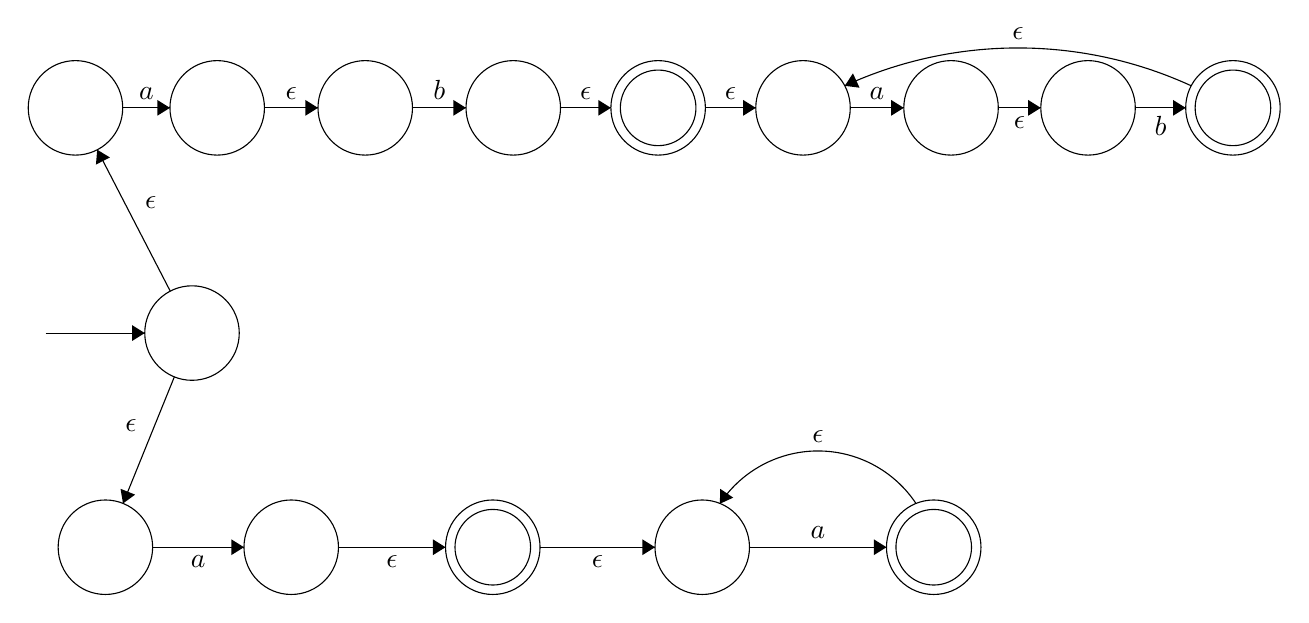
\begin{tikzpicture}[scale=0.2]
\tikzstyle{every node}+=[inner sep=0pt]
\draw [black] (3.4,-6.3) circle (3);
\draw [black] (12.4,-6.3) circle (3);
\draw [black] (21.8,-6.3) circle (3);
\draw [black] (31.2,-6.3) circle (3);
\draw [black] (40.4,-6.3) circle (3);
\draw [black] (40.4,-6.3) circle (2.4);
\draw [black] (67.7,-6.3) circle (3);
\draw [black] (76.9,-6.3) circle (3);
\draw [black] (76.9,-6.3) circle (2.4);
\draw [black] (49.6,-6.3) circle (3);
\draw [black] (59,-6.3) circle (3);
\draw [black] (10.8,-20.6) circle (3);
\draw [black] (5.3,-34.2) circle (3);
\draw [black] (17.1,-34.2) circle (3);
\draw [black] (29.9,-34.2) circle (3);
\draw [black] (29.9,-34.2) circle (2.4);
\draw [black] (43.2,-34.2) circle (3);
\draw [black] (57.9,-34.2) circle (3);
\draw [black] (57.9,-34.2) circle (2.4);
\draw [black] (6.4,-6.3) -- (9.4,-6.3);
\fill [black] (9.4,-6.3) -- (8.6,-5.8) -- (8.6,-6.8);
\draw (7.9,-5.8) node [above] {$a$};
\draw [black] (15.4,-6.3) -- (18.8,-6.3);
\fill [black] (18.8,-6.3) -- (18,-5.8) -- (18,-6.8);
\draw (17.1,-5.8) node [above] {$\epsilon$};
\draw [black] (24.8,-6.3) -- (28.2,-6.3);
\fill [black] (28.2,-6.3) -- (27.4,-5.8) -- (27.4,-6.8);
\draw (26.5,-5.8) node [above] {$b$};
\draw [black] (34.2,-6.3) -- (37.4,-6.3);
\fill [black] (37.4,-6.3) -- (36.6,-5.8) -- (36.6,-6.8);
\draw (35.8,-5.8) node [above] {$\epsilon$};
\draw [black] (70.7,-6.3) -- (73.9,-6.3);
\fill [black] (73.9,-6.3) -- (73.1,-5.8) -- (73.1,-6.8);
\draw (72.3,-6.8) node [below] {$b$};
\draw [black] (43.4,-6.3) -- (46.6,-6.3);
\fill [black] (46.6,-6.3) -- (45.8,-5.8) -- (45.8,-6.8);
\draw (45,-5.8) node [above] {$\epsilon$};
\draw [black] (52.6,-6.3) -- (56,-6.3);
\fill [black] (56,-6.3) -- (55.2,-5.8) -- (55.2,-6.8);
\draw (54.3,-5.8) node [above] {$a$};
\draw [black] (62,-6.3) -- (64.7,-6.3);
\fill [black] (64.7,-6.3) -- (63.9,-5.8) -- (63.9,-6.8);
\draw (63.35,-6.8) node [below] {$\epsilon$};
\draw [black] (52.25,-4.897) arc (114.63693:65.36307:26.387);
\fill [black] (52.25,-4.9) -- (53.19,-5.02) -- (52.77,-4.11);
\draw (63.25,-2) node [above] {$\epsilon$};
\draw [black] (1.5,-20.6) -- (7.8,-20.6);
\fill [black] (7.8,-20.6) -- (7,-20.1) -- (7,-21.1);
\draw [black] (9.42,-17.94) -- (4.78,-8.96);
\fill [black] (4.78,-8.96) -- (4.7,-9.9) -- (5.59,-9.45);
\draw (7.79,-12.31) node [right] {$\epsilon$};
\draw [black] (9.68,-23.38) -- (6.42,-31.42);
\fill [black] (6.42,-31.42) -- (7.19,-30.86) -- (6.26,-30.49);
\draw (7.31,-26.5) node [left] {$\epsilon$};
\draw [black] (8.3,-34.2) -- (14.1,-34.2);
\fill [black] (14.1,-34.2) -- (13.3,-33.7) -- (13.3,-34.7);
\draw (11.2,-34.7) node [below] {$a$};
\draw [black] (20.1,-34.2) -- (26.9,-34.2);
\fill [black] (26.9,-34.2) -- (26.1,-33.7) -- (26.1,-34.7);
\draw (23.5,-34.7) node [below] {$\epsilon$};
\draw [black] (32.9,-34.2) -- (40.2,-34.2);
\fill [black] (40.2,-34.2) -- (39.4,-33.7) -- (39.4,-34.7);
\draw (36.55,-34.7) node [below] {$\epsilon$};
\draw [black] (46.2,-34.2) -- (54.9,-34.2);
\fill [black] (54.9,-34.2) -- (54.1,-33.7) -- (54.1,-34.7);
\draw (50.55,-33.7) node [above] {$a$};
\draw [black] (44.316,-31.437) arc (146.51092:33.48908:7.475);
\fill [black] (44.32,-31.44) -- (45.17,-31.05) -- (44.34,-30.49);
\draw (50.55,-27.59) node [above] {$\epsilon$};
\end{tikzpicture}
\end{center}

\problem{1.29}
Use the pumping lemma to show that the following languages are not regular. \\  \\
\problem{1.29 b} 
$A_2 = \{www| w \in \{a,b\}^*\}$\\ \\
\answ{Assume} that $A_2 = \{www| w \in \{a,b\}^*\}$ is regular. Let p be the pumping 
length given by the pumping lemma. Choose $s$ to be the string $a^pba^pba^pb$. 
Because s is a member of $A_2$ and $s$ is longer than p, the pumping lemma guarantees 
that $s$ can be split into three pieces, $s=xyz$, where $|xy| \leq p$, hence $y$ can 
only be contained in first $a^p$. Since $y \geq 1$, let $y = a^i$, $i > 0$. 
However, $xy^2z = a^{p+k}ba^pba^pb$, where $p+k > P$, is not in $A_2$. That is $s$ 
cannot be pumped. This is a contradiction. Thus, $A_2$ is not regular.

\vspace{1cm}
\problem{1.31}
For any string $ w = w_qw_2\cdot w_n$, the reverse of $w$, written $w^R$, is the string $w$ in reverse order, 
$w_n\cdots w_2 w_1$.  For any language $A$, let $A^R = \{w^R | w \in A\}$.
Show that if $A$ is regular, so is $A^R$.\\ \\
\answ{By} theorem if $A$ is regular, then there is a DFA $M = (Q,\sum, \delta, q_0, F)$ such that $M$ recognizes $A$. 
We will show that it is possible to construct
an NFA $N = (Q',\sum ', \delta ', q_0 ', F ')$ that will recognize $A^R$. \\

Informally:
\begin{enumerate}[1., leftmargin = 0.5cm, nosep]
\item Reverse all the connections in the automaton.
\item Add a new state $q_f$
\item Draw $\epsilon$ connection from state $q_f$ to every final state.
\item Make all the final states normal states.
\item Make start state final state.
\item Make $q_f$ the start state. \\
\end{enumerate}
Formally
\begin{itemize}
\item New set of states $Q' = Q \cup \{q_0'\}$, where $q_0$ is the new start state
\item New set of final states $F' = \{q_0\}$ 
i.e. we will accept only in the start state of the original DFA.
\item New transition function $\delta'$ is definde as follows
\begin{equation}
  \delta(q,a) '=\begin{cases}
    F, & \text{if } q = q_0' \text{ and } a = \epsilon \\
    \delta^{-1}(q,a), & \text{if } q \neq q_0' \text{ and } a \neq \epsilon . \\
    \emptyset, & \text{otherwise}.
  \end{cases}
\end{equation}

\end{itemize}
$\delta$ $q_0, q_1, \cdots, q_n$ is in accepting computation of $M$ on input $w_1w_2\cdots w_n$ if
and only if $\delta'$ $q_n,\cdots ,q_1, q_0 $ is an accepting computation of $N$ on input $w_n \cdots w_2 w_1$ (since
$\delta(q_i,w_{i+1} = q_{i+i}$ iff $q_i \in \delta' (q_{i+1},w_{i+1})$ for $0 \leq i < n$ and 
$q_n \in \delta'(q_0', \epsilon))$. Thus, $N$ recognizes $A^R$. Therefore for any regular language $A$ there exists an NFA that recognizes
$A^R$.\\

\vspace{1cm}
\problem{1.32}

Let $w^R$ denote the reverse of the string $w$. For any language A, let $A^R = \{w^R | w\in A\}$.
Then if $A$ is regular, so is $A^R$.
\\
Now, the construction of the automata for the language $B^R$ is simple. We get columns of size 3
as our alphabets at each stage, we will need to keep track of two things, wheter there is a carry or not. Depending on wheter there
was a carry or not, we just need to verify that the provided 3-column is consistent. \\
$a = 
\begin{bmatrix}
    0 \\
    0 \\
    0  
\end{bmatrix}
\begin{bmatrix}
    1 \\
    0 \\
    1  
\end{bmatrix}
\begin{bmatrix}
    0 \\
    1 \\
    1  
\end{bmatrix}
$
$b = 
\begin{bmatrix}
    1 \\
    1 \\
    0  
\end{bmatrix}
$
$c = 
\begin{bmatrix}
    0 \\
    1 \\
    0  
\end{bmatrix}
\begin{bmatrix}
    1 \\
    0 \\
    0  
\end{bmatrix}
\begin{bmatrix}
    1 \\
    1 \\
    1  
\end{bmatrix}
$
$d = 
\begin{bmatrix}
    0 \\
    0 \\
    1  
\end{bmatrix}
$
\begin{center}
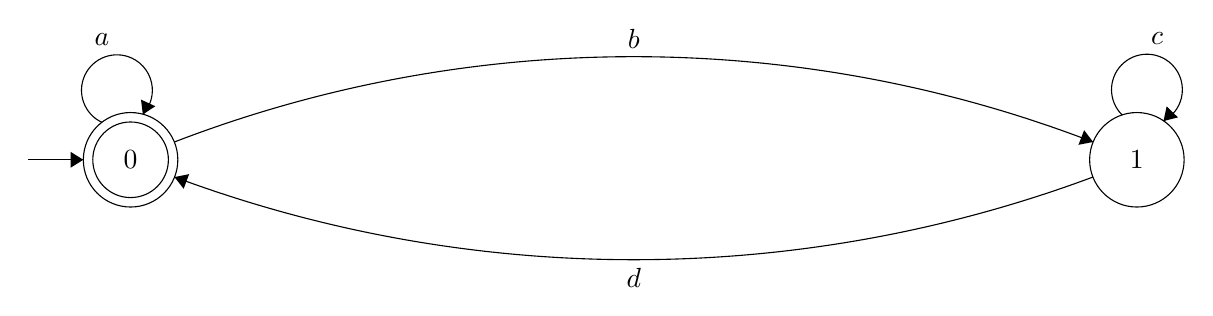
\begin{tikzpicture}[scale=0.2]
\tikzstyle{every node}+=[inner sep=0pt]
\draw [black] (8.5,-12.2) circle (3);
\draw (8.5,-12.2) node {$0$};
\draw [black] (8.5,-12.2) circle (2.4);
\draw [black] (72.4,-12.2) circle (3);
\draw (72.4,-12.2) node {$1$};
\draw [black] (11.279,-11.071) arc (111.05434:68.94566:81.198);
\fill [black] (69.62,-11.07) -- (69.05,-10.32) -- (68.69,-11.25);
\draw (40.45,-5.15) node [above] {$b$};
\draw [black] (6.686,-9.826) arc (245.11724:-42.88276:2.25);
\draw (6.68,-4.99) node [above] {$a$};
\fill [black] (9.28,-9.32) -- (10.07,-8.8) -- (9.16,-8.38);
\draw [black] (71.472,-9.36) arc (225.82862:-62.17138:2.25);
\draw (73.69,-4.93) node [above] {$c$};
\fill [black] (74.09,-9.74) -- (75.01,-9.51) -- (74.29,-8.81);
\draw [black] (2,-12.2) -- (5.5,-12.2);
\fill [black] (5.5,-12.2) -- (4.7,-11.7) -- (4.7,-12.7);
\draw [black] (69.608,-13.297) arc (-69.58366:-110.41634:83.585);
\fill [black] (11.29,-13.3) -- (11.87,-14.04) -- (12.22,-13.11);
\draw (40.45,-19.05) node [below] {$d$};
\end{tikzpicture}
\end{center}

\pagebreak

\problem{1.46}
Prove tat the following languages are not regular. You may use the pumping lemma and the closure of the class of regular
languages under union, intersection and compliment.\\ \\
\problem{1.46 c}\\
$L = \{w|w \in \{0,1\}^* \text{ is not a palindrome }\}$ \\

We can show that $L$ is not regular, by showing that it's compliment
$L' = \{w|w \in \{0,1\}^* \text{ is a palindrome }\}$ is not regular. \\
Choose $s = 0^p10^p = xyz,\text{ a palindrome in } L'$. Here $xy$ contains only 0's, since $xy \leq p$.
Let $y = 0^k$, should be in the language for  all $k \geq 0$, however $xy^0z = 0^{p-k}10^p$ is not in the language. 
Thus, $L'$ is not regular, therefore $L$ is not regular as well.


%\begin{homeworkProblem}
%\end{homeworkProblem}
\end{document}
